\documentclass{article}
\usepackage{graphicx}
\usepackage{amsmath}
\usepackage{listings}
\usepackage{float}
\usepackage[margin=1in]{geometry}

\title{CS2323 Computer Architecture\\Mid-Term Submission - RISC-V Processor Implementation}
\author{Abhimanyu Koushik Garimella\\EE24BTECH11024}
\date{October 2025}

\lstset{
    basicstyle=\ttfamily\small,
    breaklines=true,
    frame=single,
}

\begin{document}

\maketitle

\section*{Introduction}

This document details the progress on the RV64IMD processor implementation project. The focus has been on designing and implementing the core datapath components. These fundamental building blocks form the foundation of the non-pipelined baseline processor that will eventually be extended to support the full RV64IMD instruction set with pipelining. The complete datapath designed for a single-cycle processor is presented below.

\section*{Arithmetic and Logic Unit}

\begin{figure}[H]
    \centering
    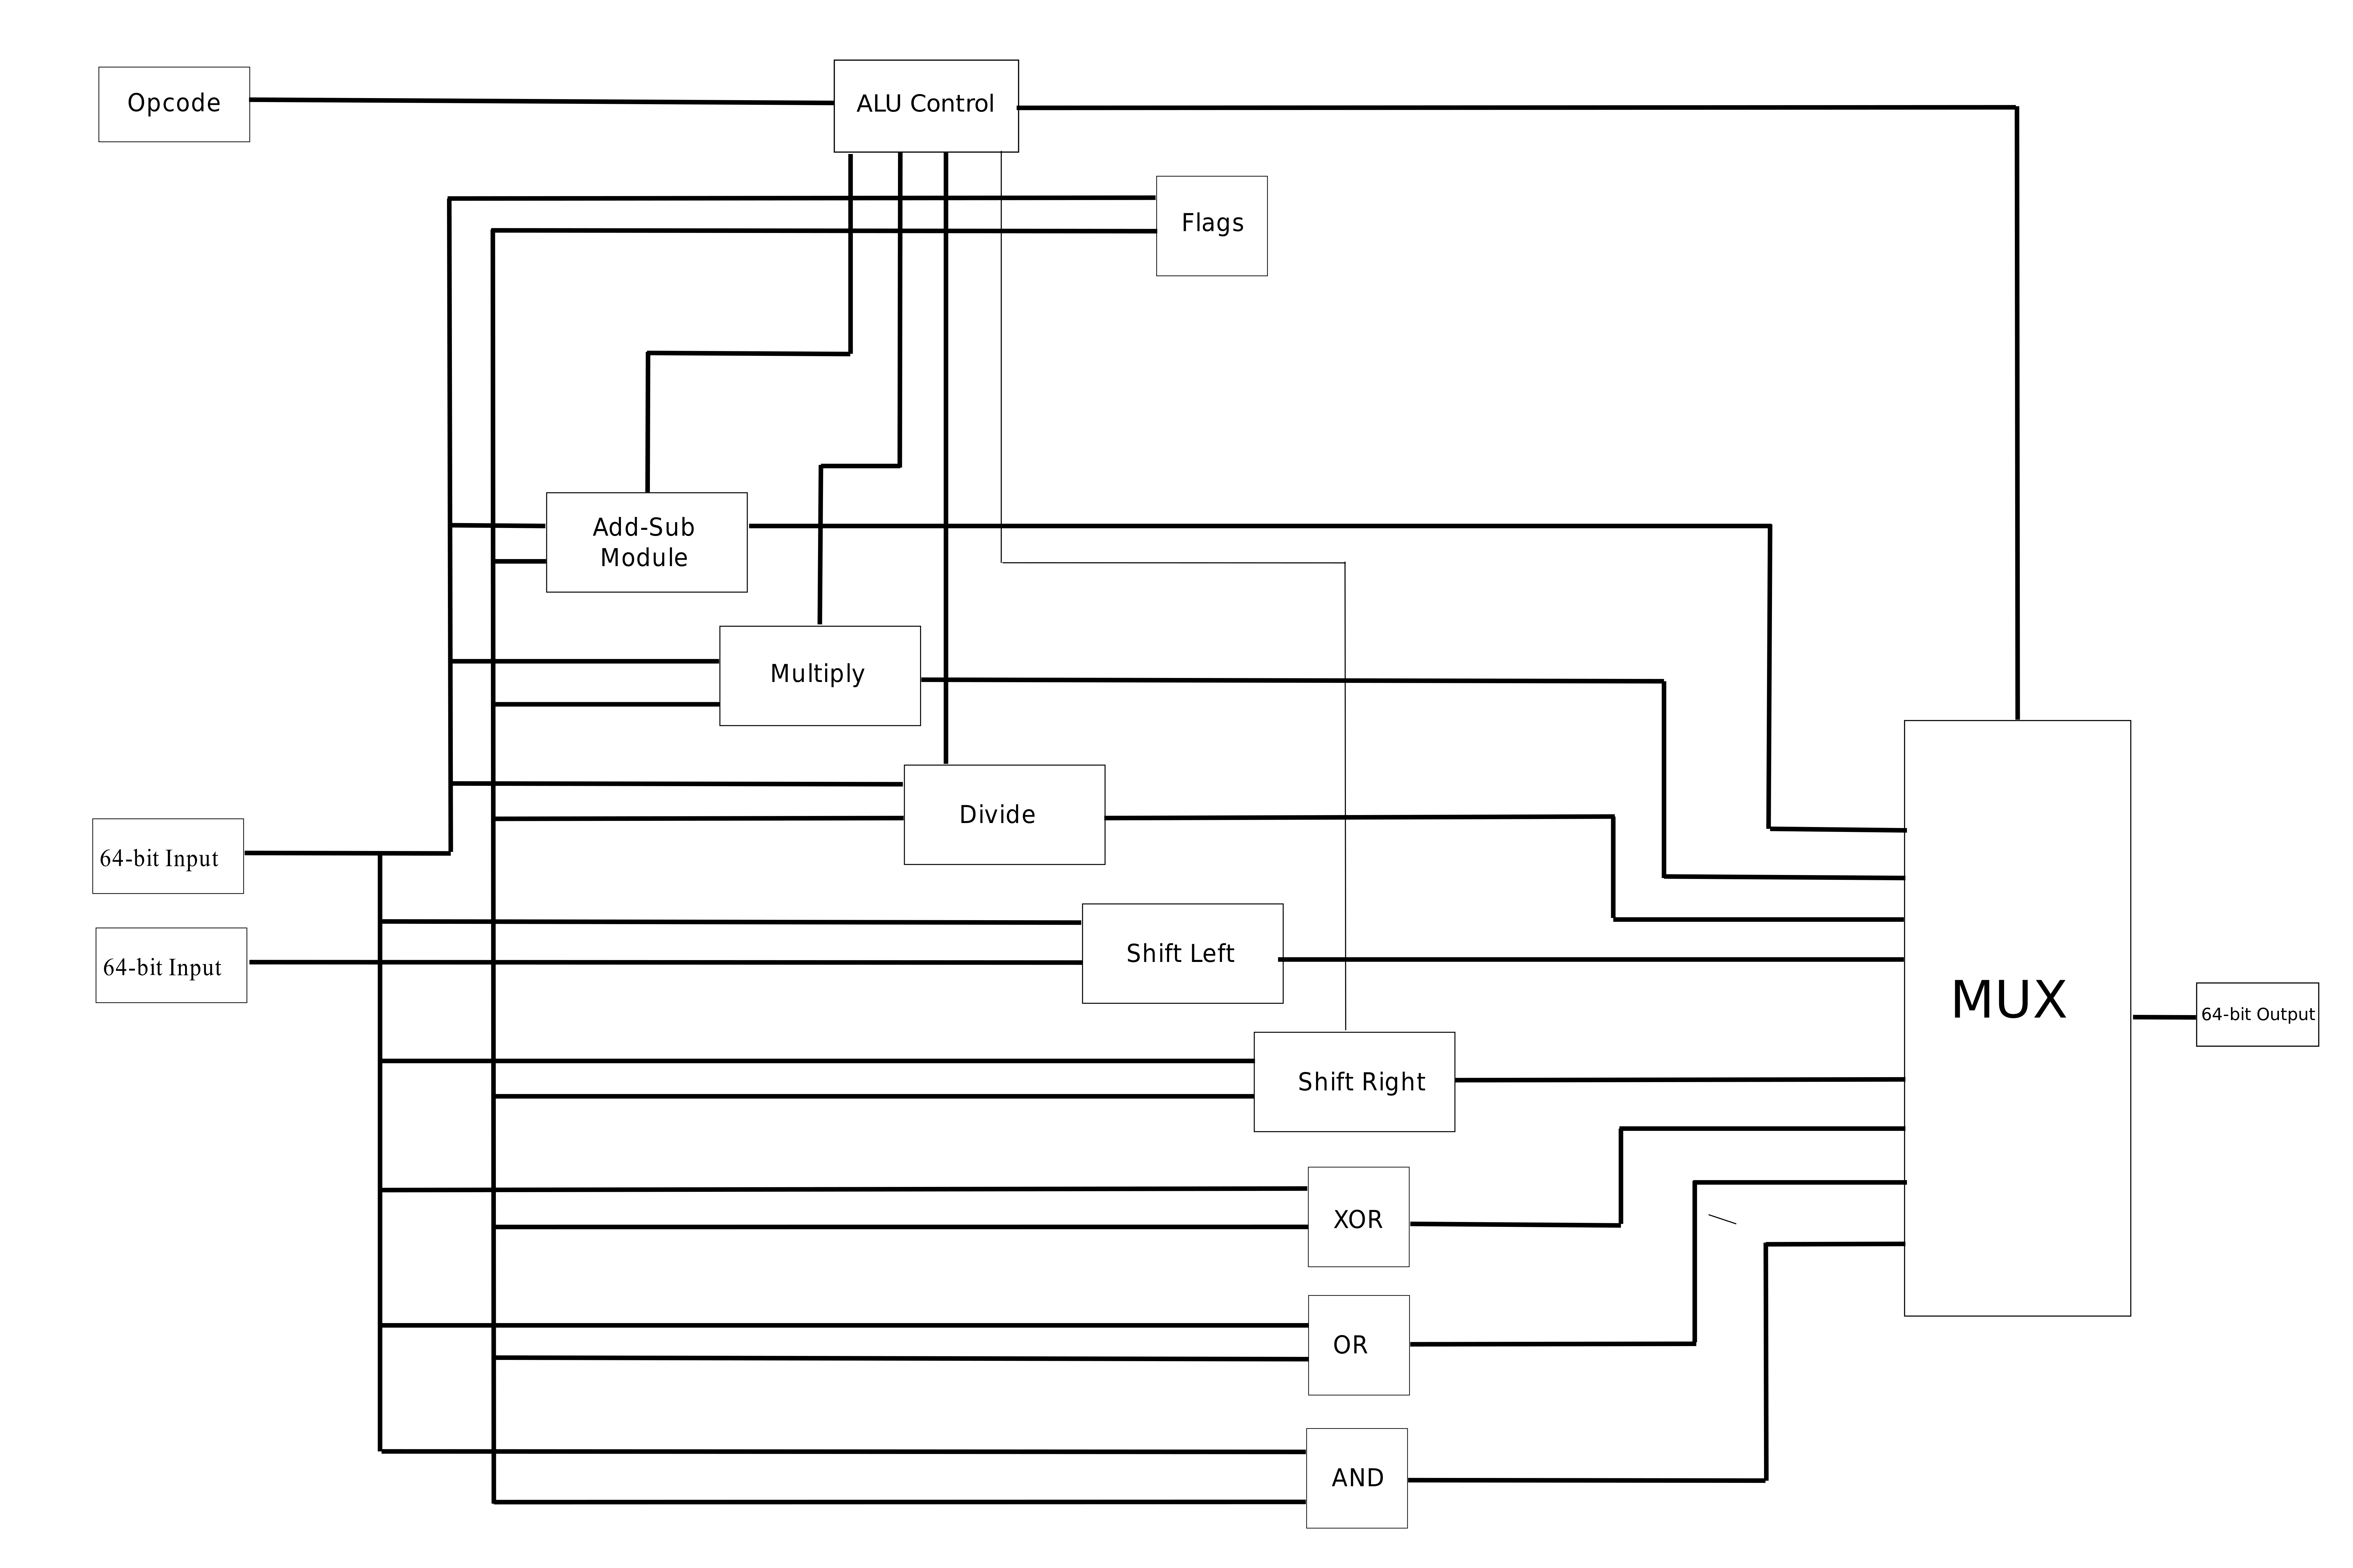
\includegraphics[width=\linewidth]{ALU.png}
    \caption{ALU Block}
    \label{fig:alu}
\end{figure}

The task of the ALU is to take the input values from the input ports, perform the specific operation specified by the ALUOp, and send back the output. All operations specified in the RISC-V instruction set are implemented. Each operation was performed directly in Verilog using the provided operations, with careful consideration given to understanding how each operation is implemented. The output for all operations is calculated simultaneously, and a final multiplexer is used to select the correct output, with the select lines for the multiplexer being the ALUOp codes.

\subsection*{Addition-Subtraction Block}

The task of the Addition-Subtraction block is to perform addition, subtraction, set less than, and set less than unsigned operations. For addition and subtraction, a basic 64-bit addition block is used. One of the inputs is taken directly from the inputs of the ALU, while the other input is selected by a multiplexer whose inputs are the second input and its negative. The select line for the multiplexer comes from the ALU Control.

\begin{figure}[H]
    \centering
    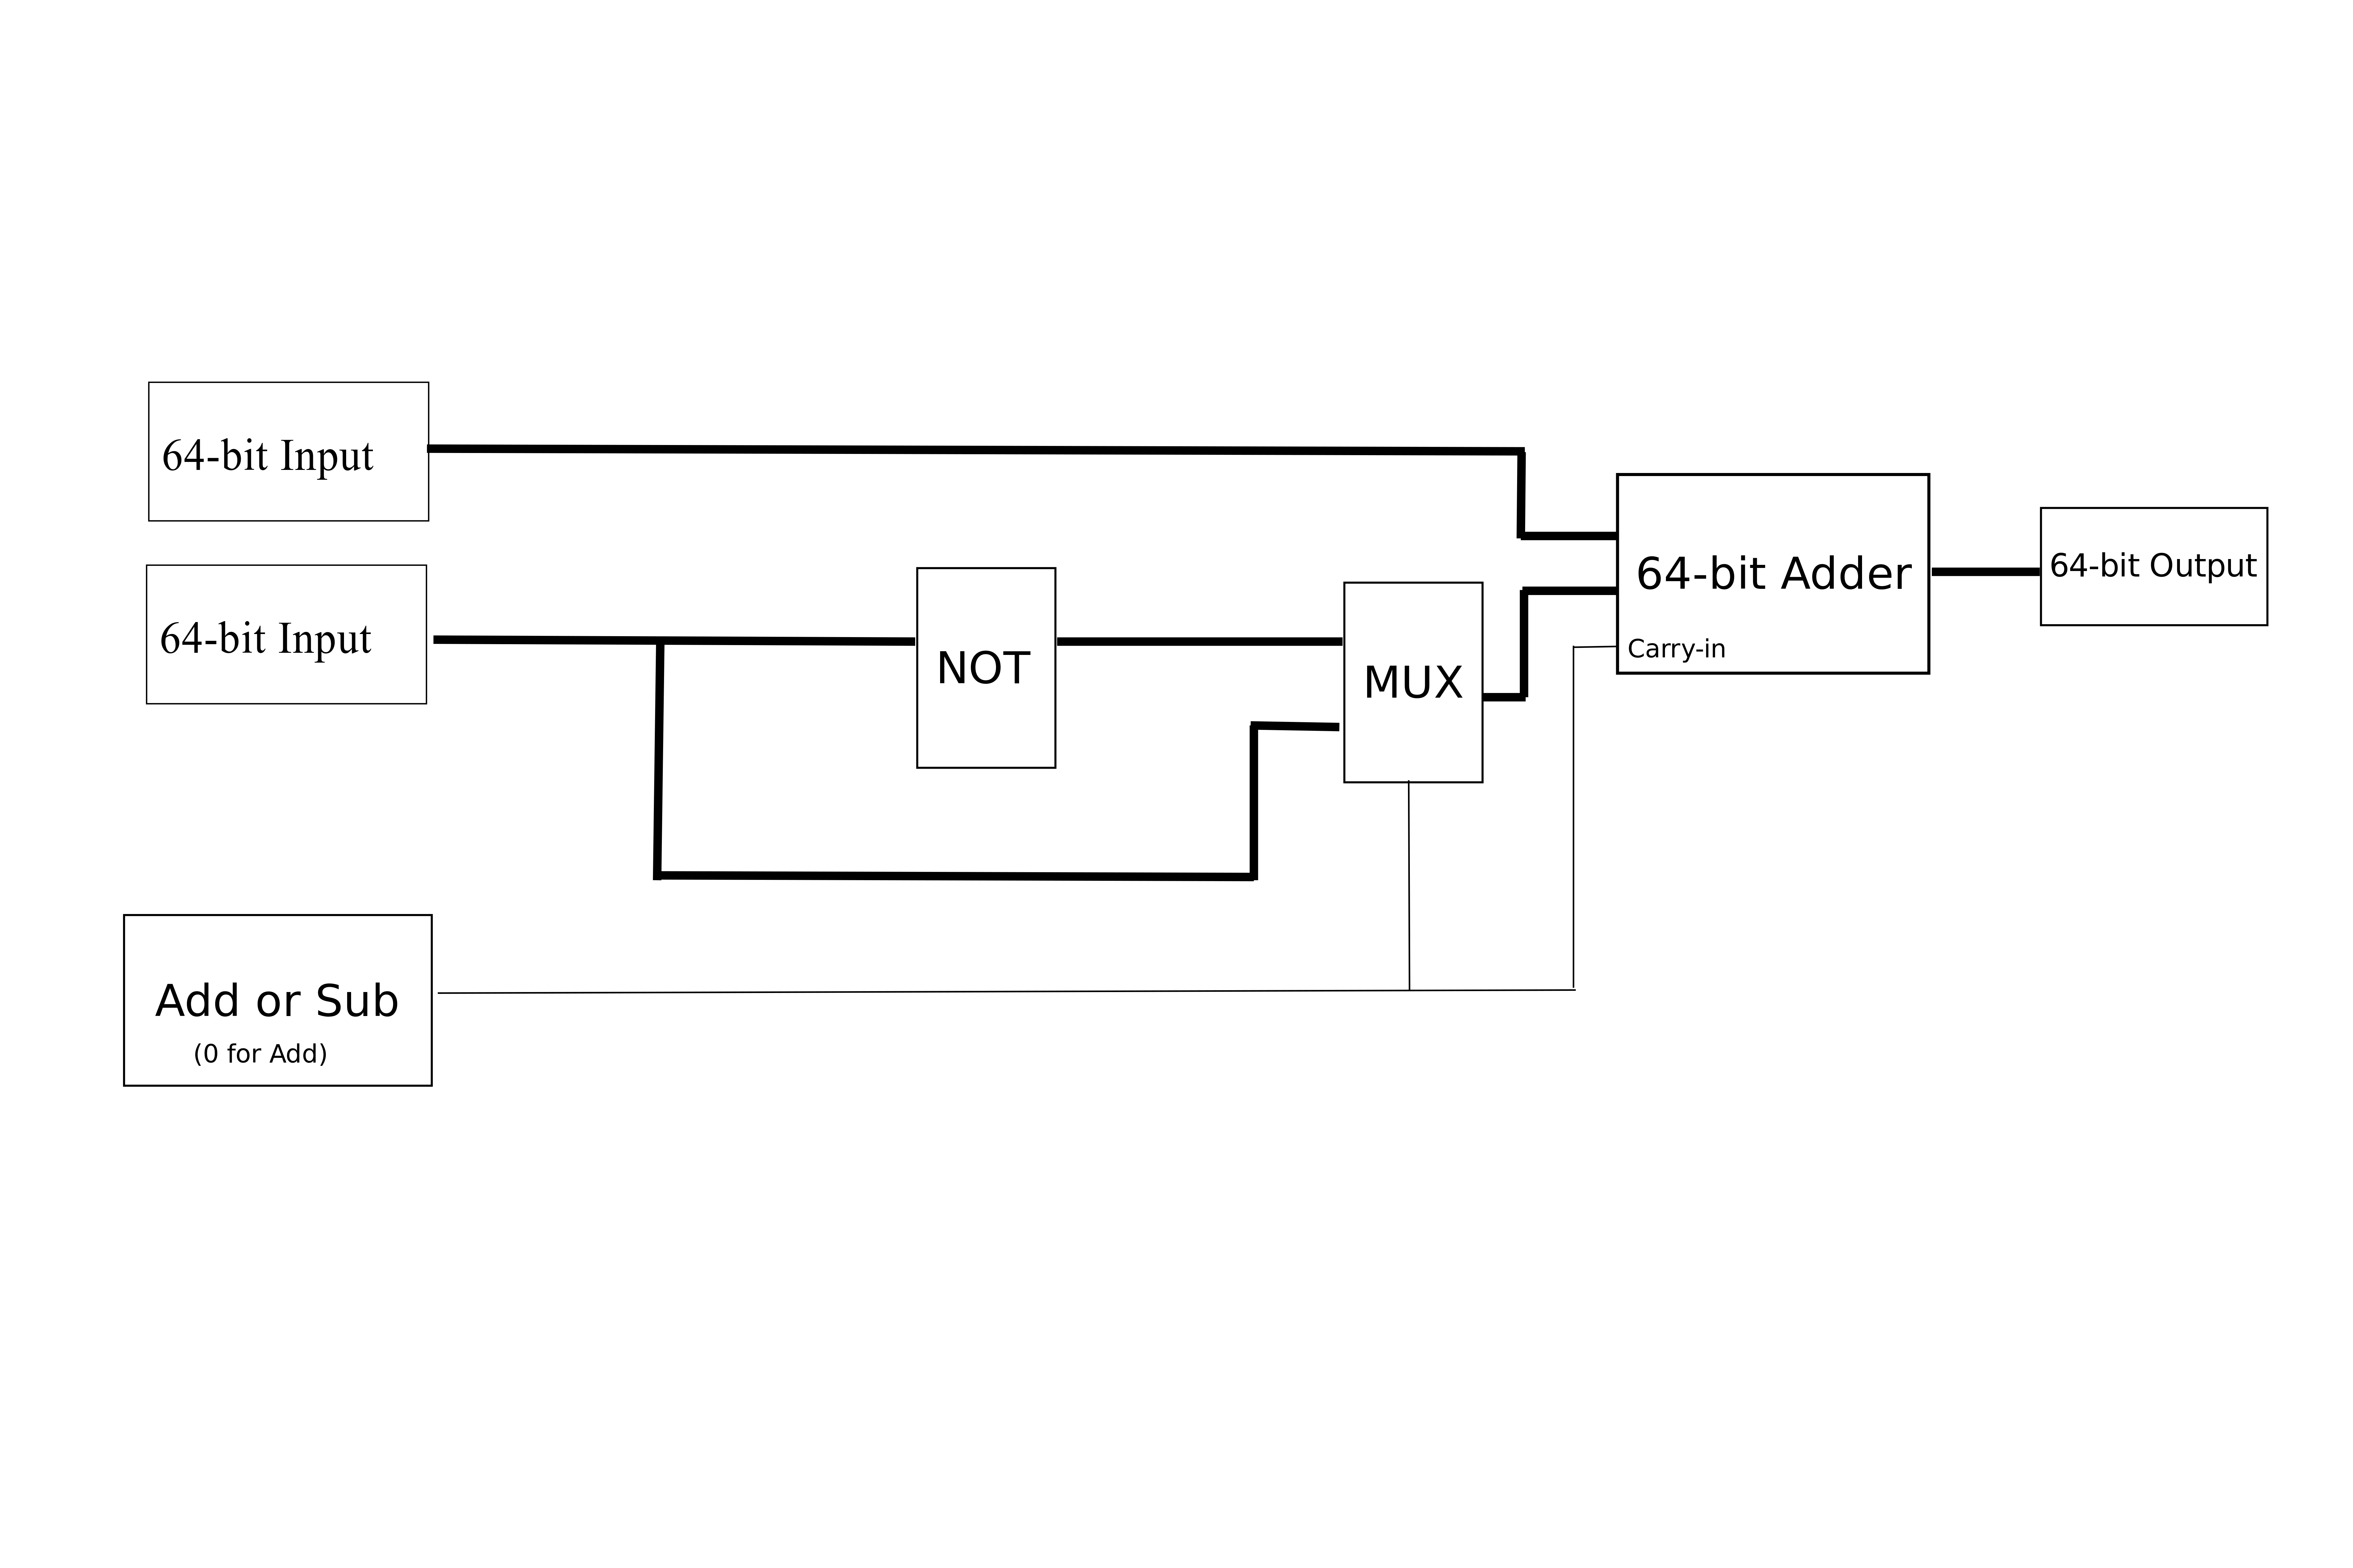
\includegraphics[width=\linewidth]{Addsub.png}
    \caption{Addition-Subtraction Block}
    \label{fig:addsub}
\end{figure}

\subsection*{Shift Operations}

Shift operations are essential for bit manipulation and multiplication/division by powers of 2. The RISC-V ISA specifies three types of shifts: logical left, logical right, and arithmetic right.

The shift left operation performs logical left shifts by inserting zeros from the right. For a 64-bit operand, the shift amount ranges from 0 to 63 bits. It was designed as shown below.

\begin{figure}[H]
    \centering
    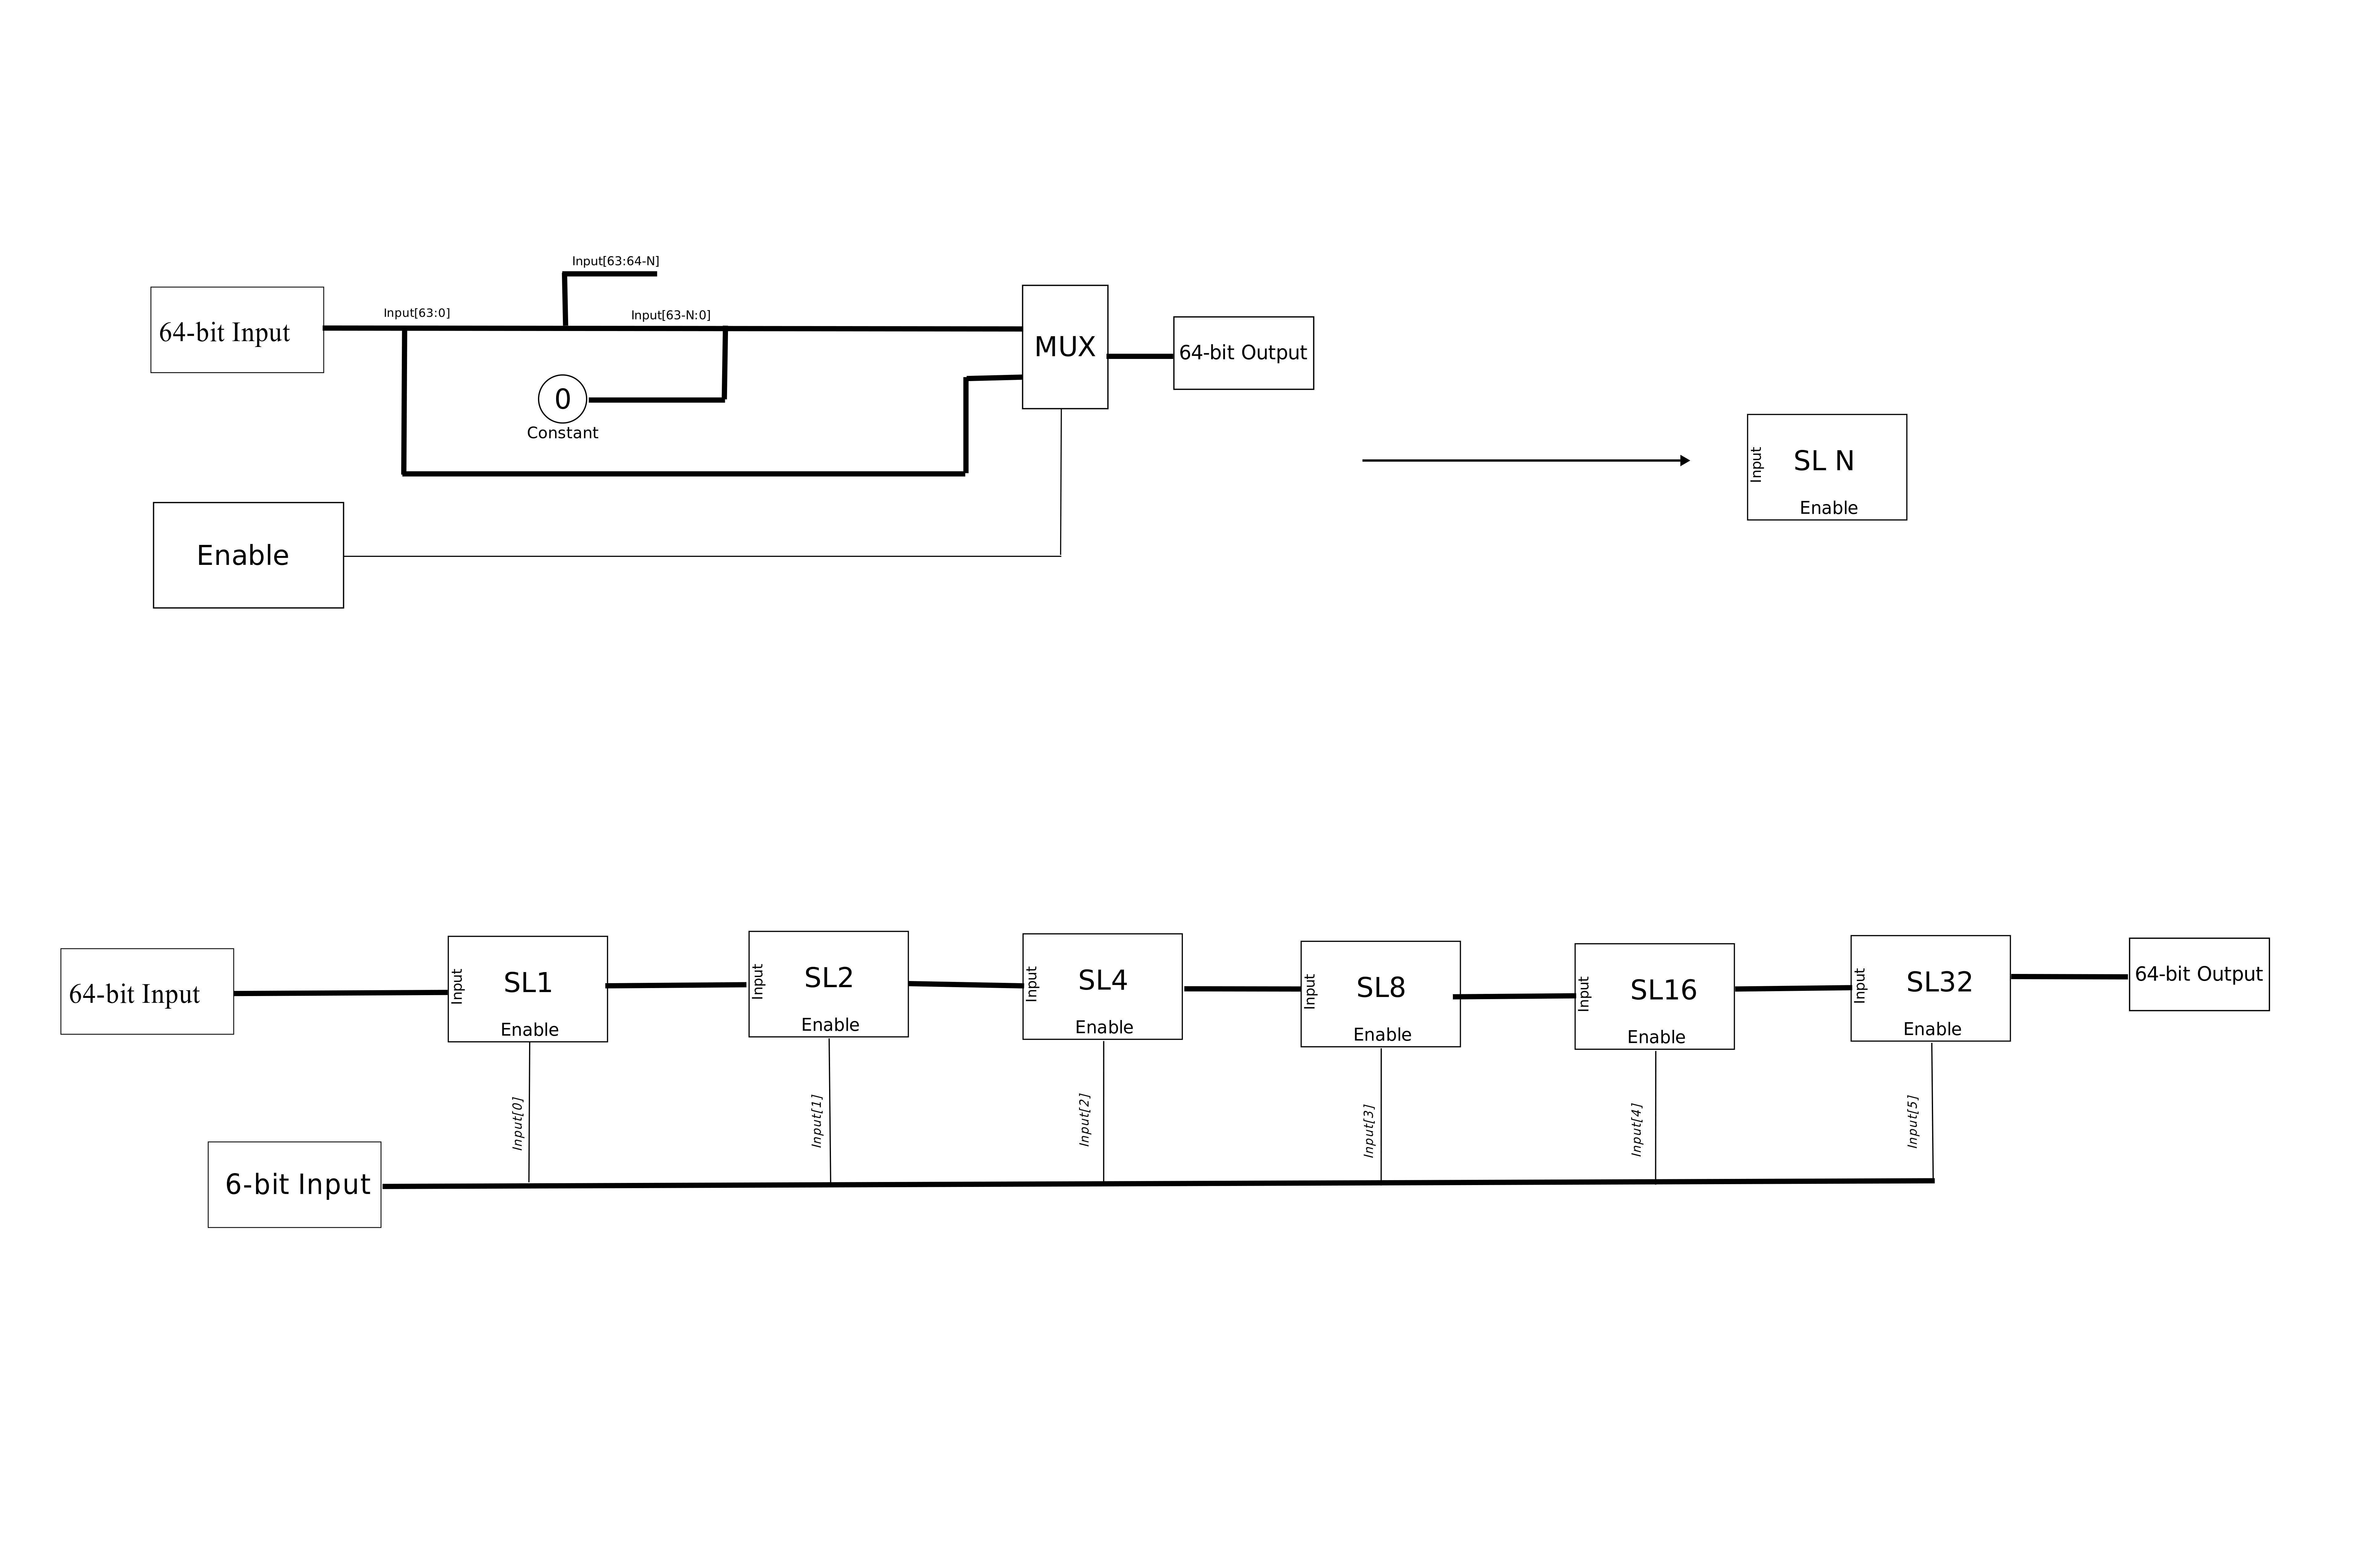
\includegraphics[width=\linewidth]{ShiftLeft_nbits.png}
    \caption{Shift Left Block}
    \label{fig:shiftleft}
\end{figure}

The shift right operation performs logical right shifts by inserting zeros or ones from the left. For a 64-bit operand, the shift amount ranges from 0 to 63 bits. It was designed as shown below.

\begin{figure}[H]
    \centering
    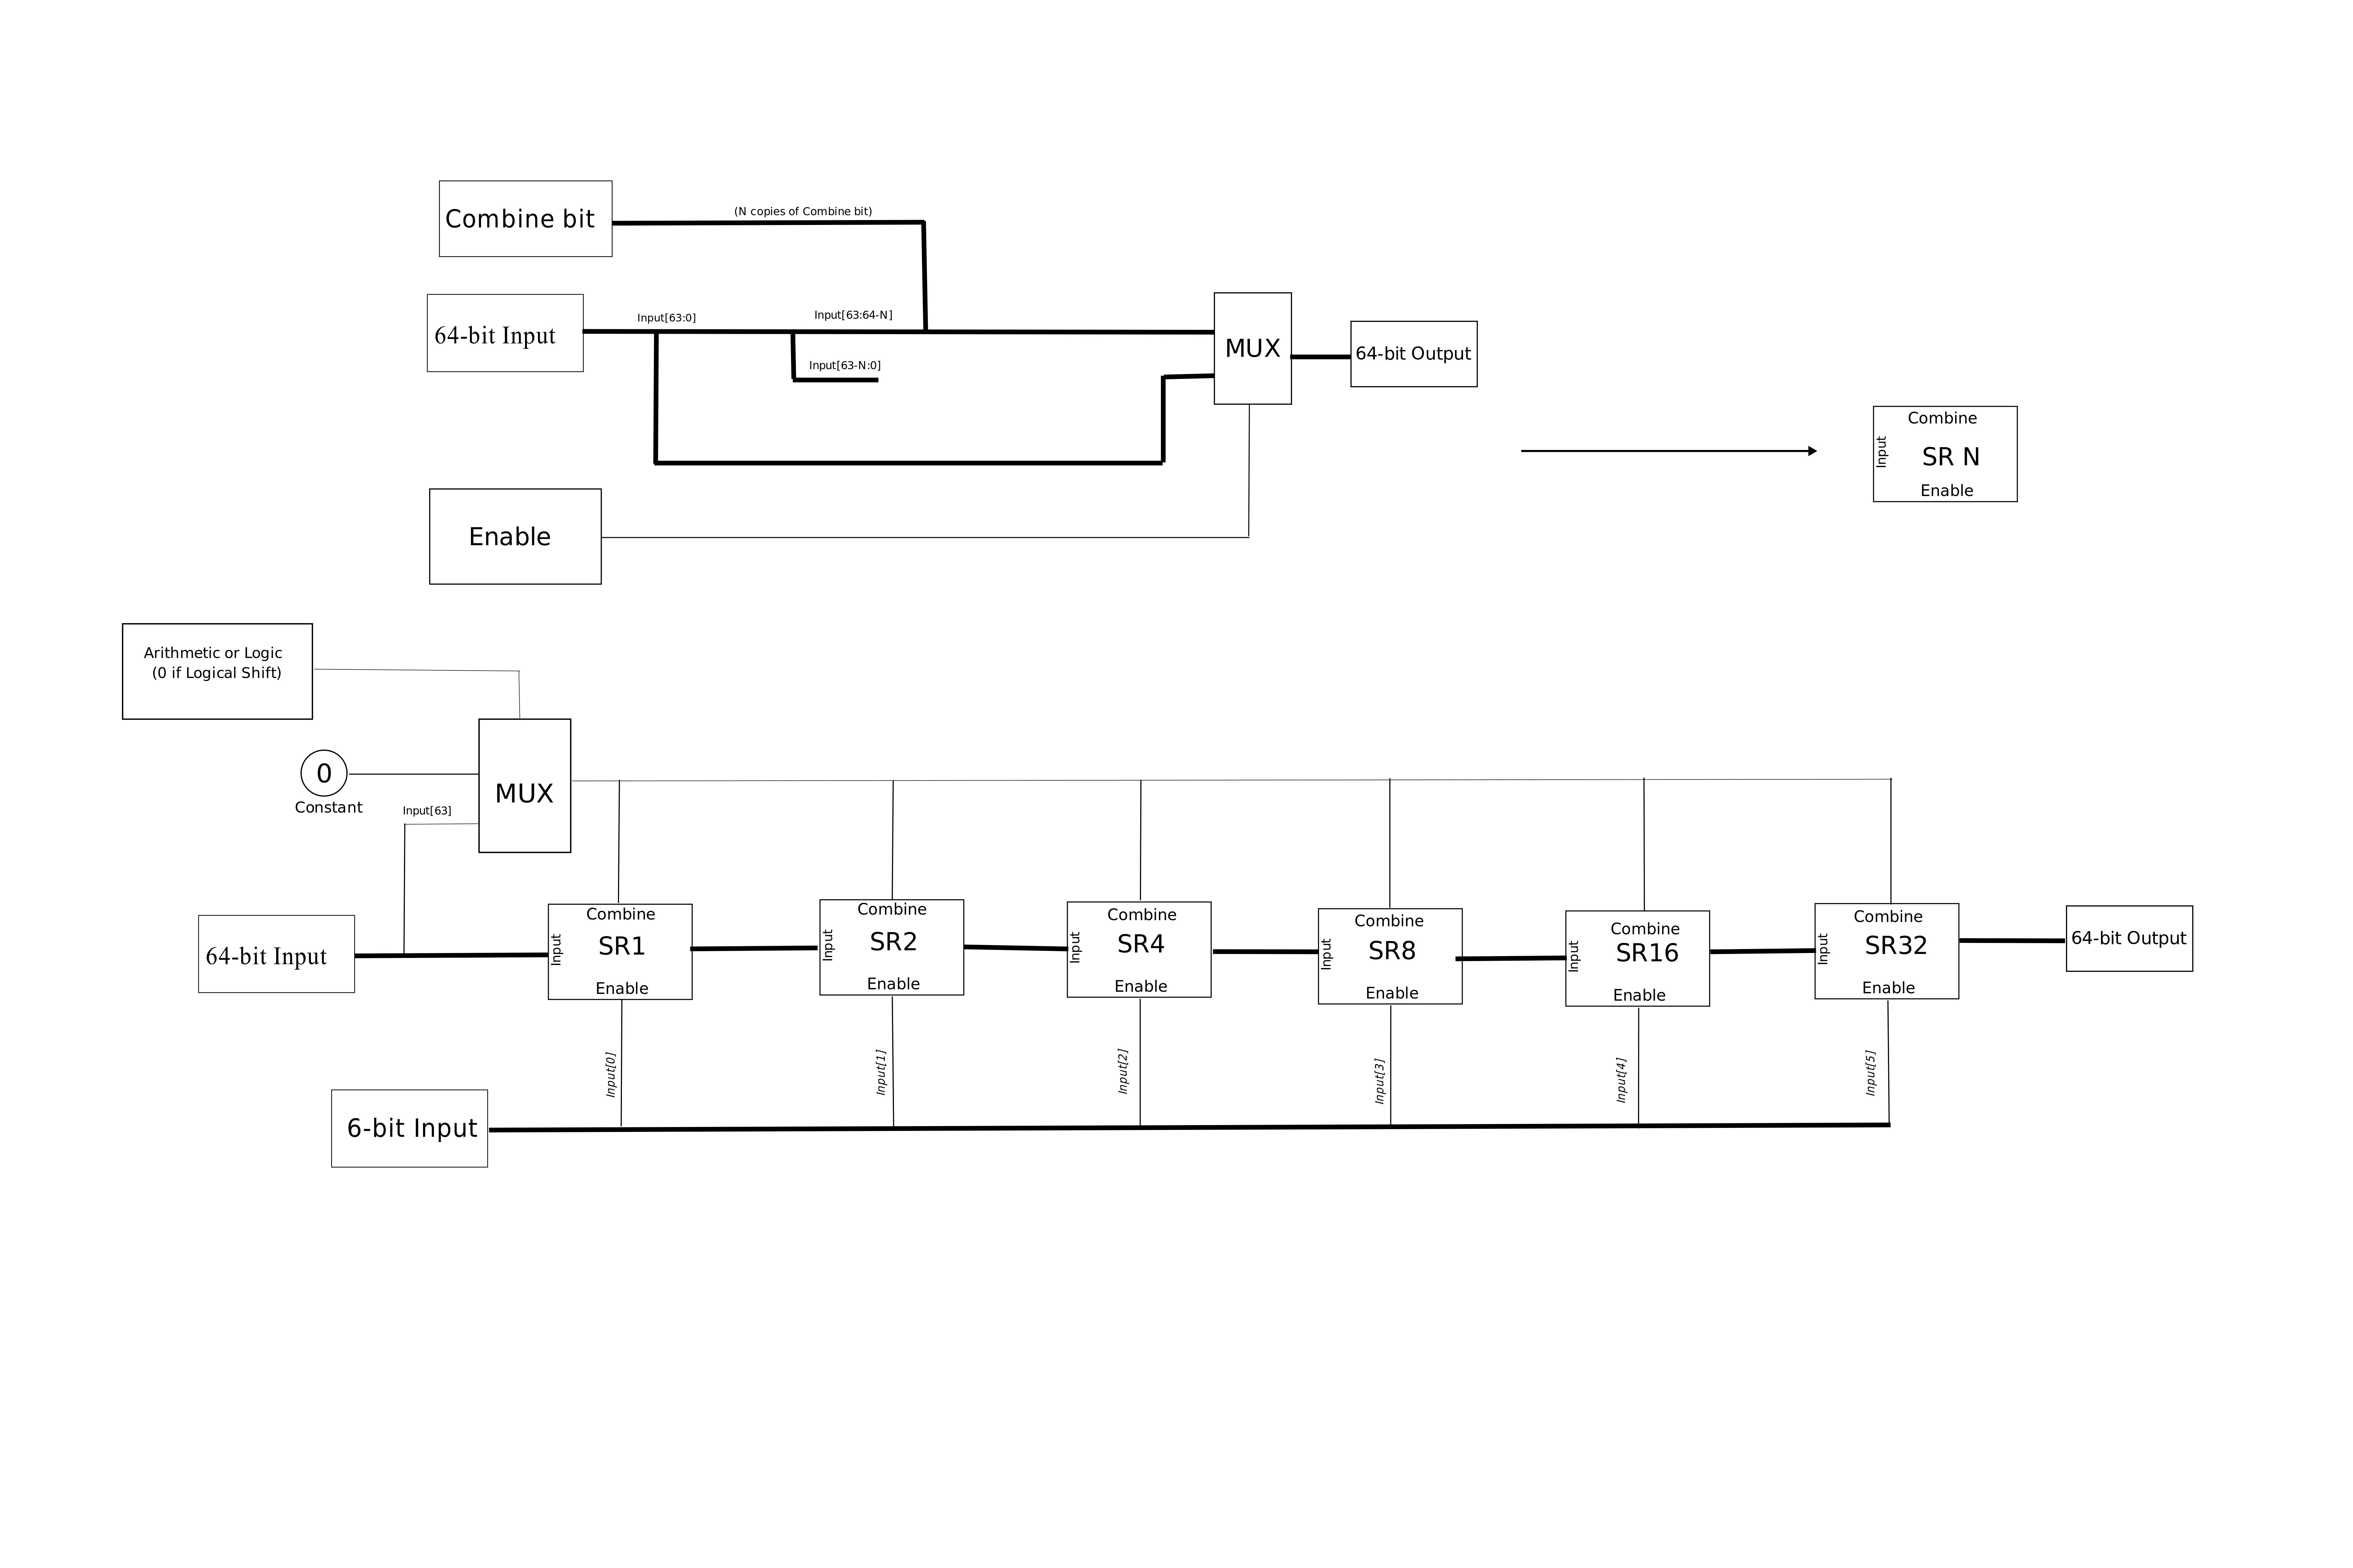
\includegraphics[width=\linewidth]{Shiftright_nbits.png}
    \caption{Shift Right Block}
    \label{fig:shiftright}
\end{figure}

A control signal selects between logical and arithmetic mode. For arithmetic shifts, the most significant bit is used as the fill value.

\subsection*{Unsigned Multiplier}

The M-extension of RISC-V requires hardware multiplication support. The multiplier unit implements unsigned multiplication for 64-bit operands.

The multiplier uses an iterative add-and-shift algorithm. For two \(n\)-bit numbers \(A\) and \(B\), the product is computed as:
\[
P = \sum_{i=0}^{n-1} A \cdot B_i \cdot 2^i
\]
where \(B_i\) is the \(i\)-th bit of \(B\).

\begin{figure}[H]
    \centering
    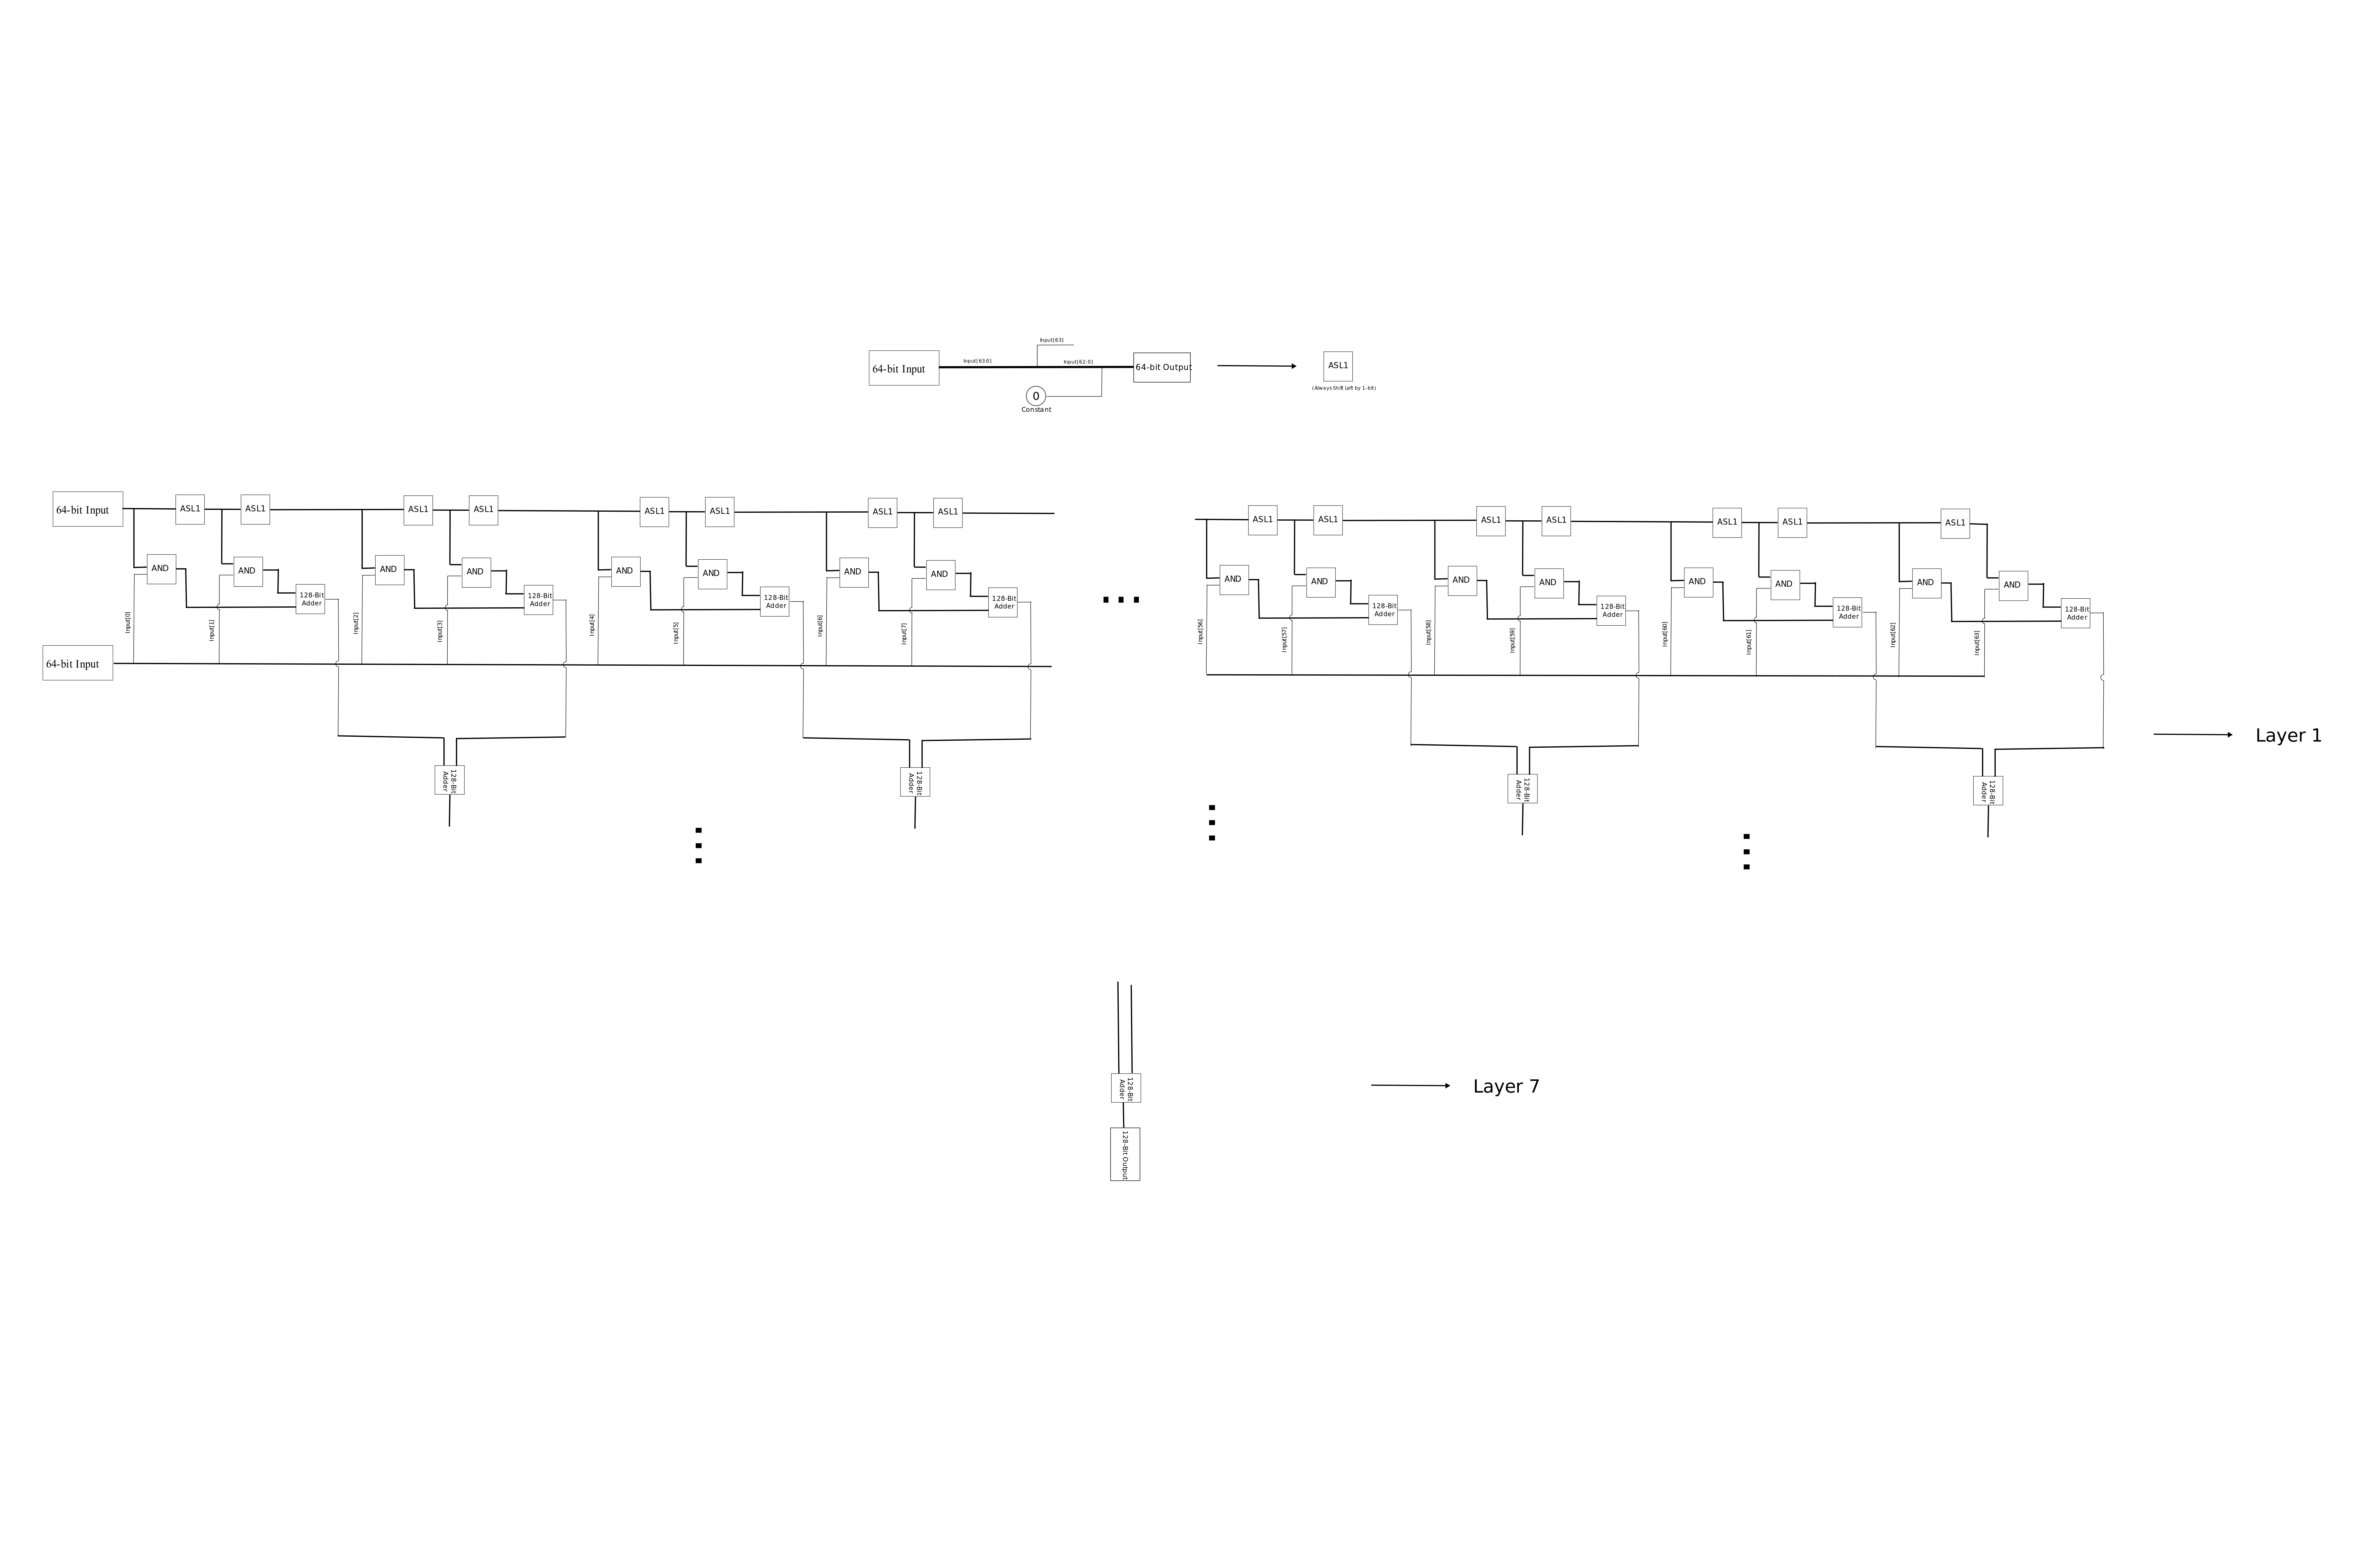
\includegraphics[width=0.7\textwidth]{Unsigned_multiplier.png}
    \caption{Unsigned Multiplier Architecture}
    \label{fig:multiplier}
\end{figure}
Once all the partial sums are calculated, they are added in parallel manner.

For signed multiplication (MULH, MULHSU), the operands are converted to unsigned values, multiplied, and the result is adjusted based on the original signs.

\subsection*{Unsigned Divider}

Division is more complex than multiplication and requires careful handling of edge cases. The divider implements unsigned division and produces both quotient and remainder.

The divider uses a restoring division algorithm. For dividend \(N\) and divisor \(D\), it computes quotient \(Q\) and remainder \(R\) such that:
\[
N = Q \cdot D + R, \quad 0 \leq R < D
\]

\begin{figure}[H]
    \centering
    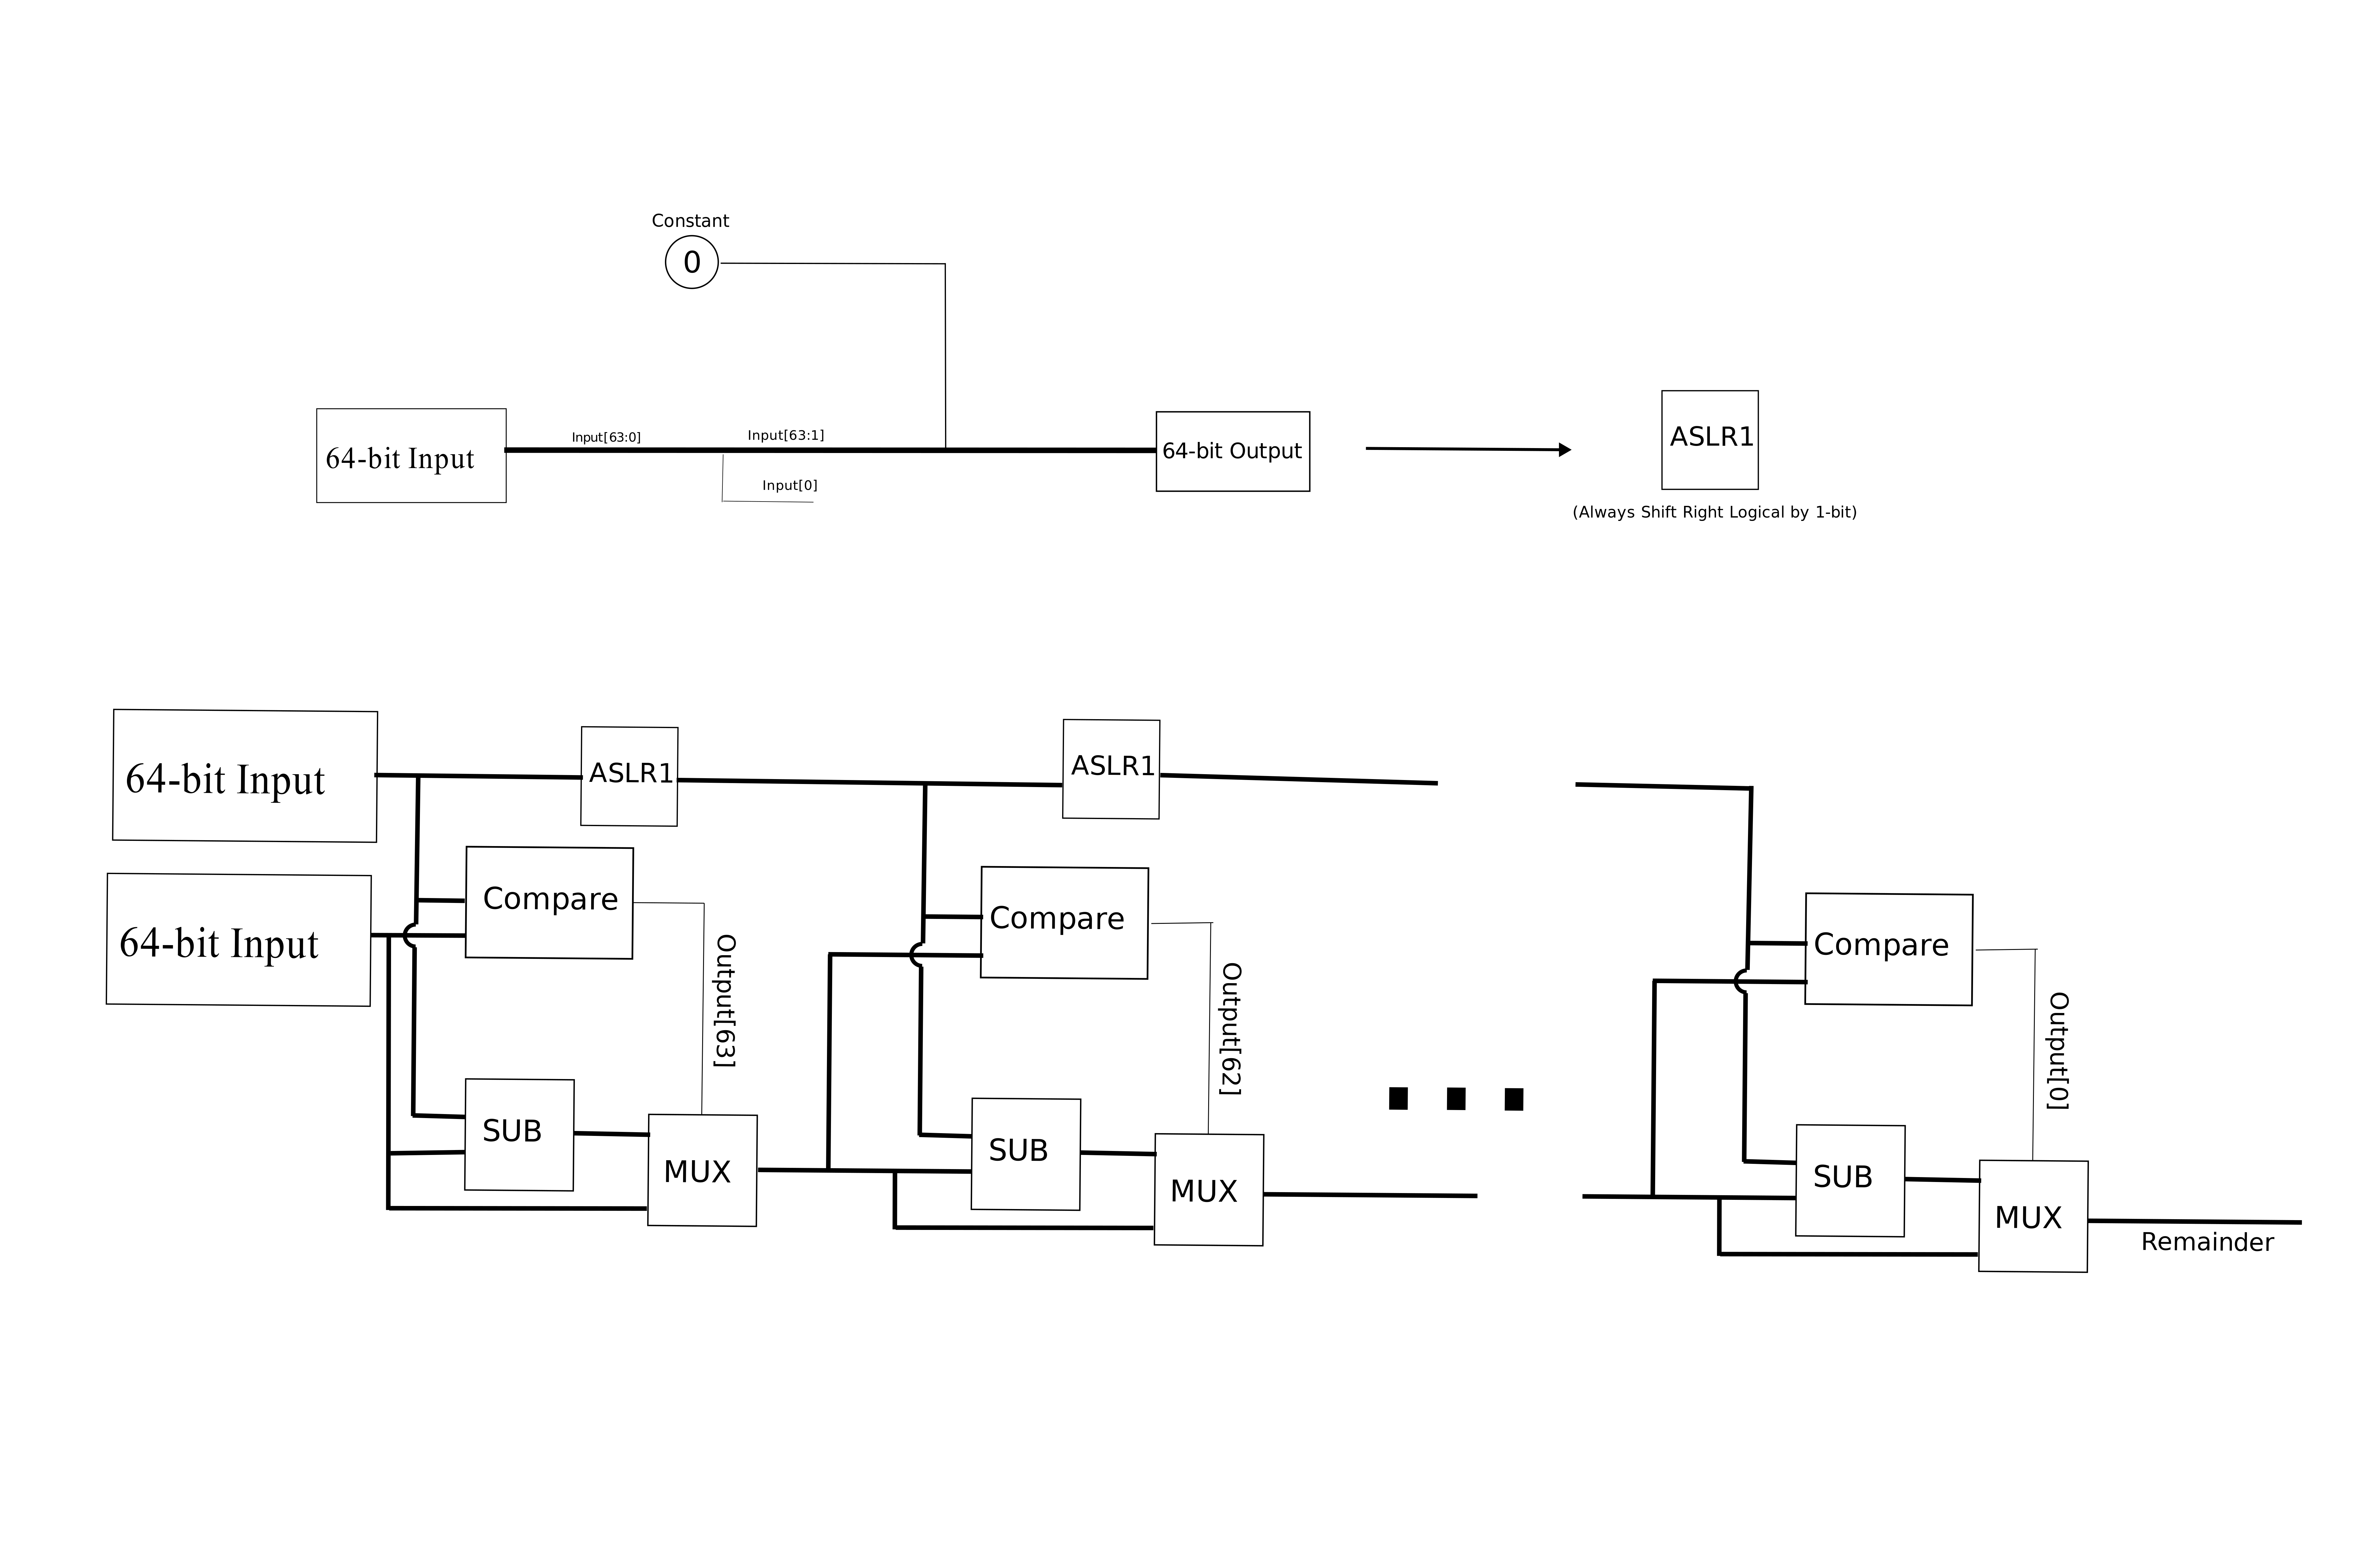
\includegraphics[width=0.7\textwidth]{Unsigned_divider.png}
    \caption{Unsigned Divider Architecture}
    \label{fig:divider}
\end{figure}

The algorithm works by repeatedly subtracting the divisor from the dividend. If the subtraction produces a non-negative result, a 1 is placed in the quotient and the remainder is updated. Otherwise, a 0 is placed in the quotient and the remainder is restored.

\begin{figure}
    \centering
    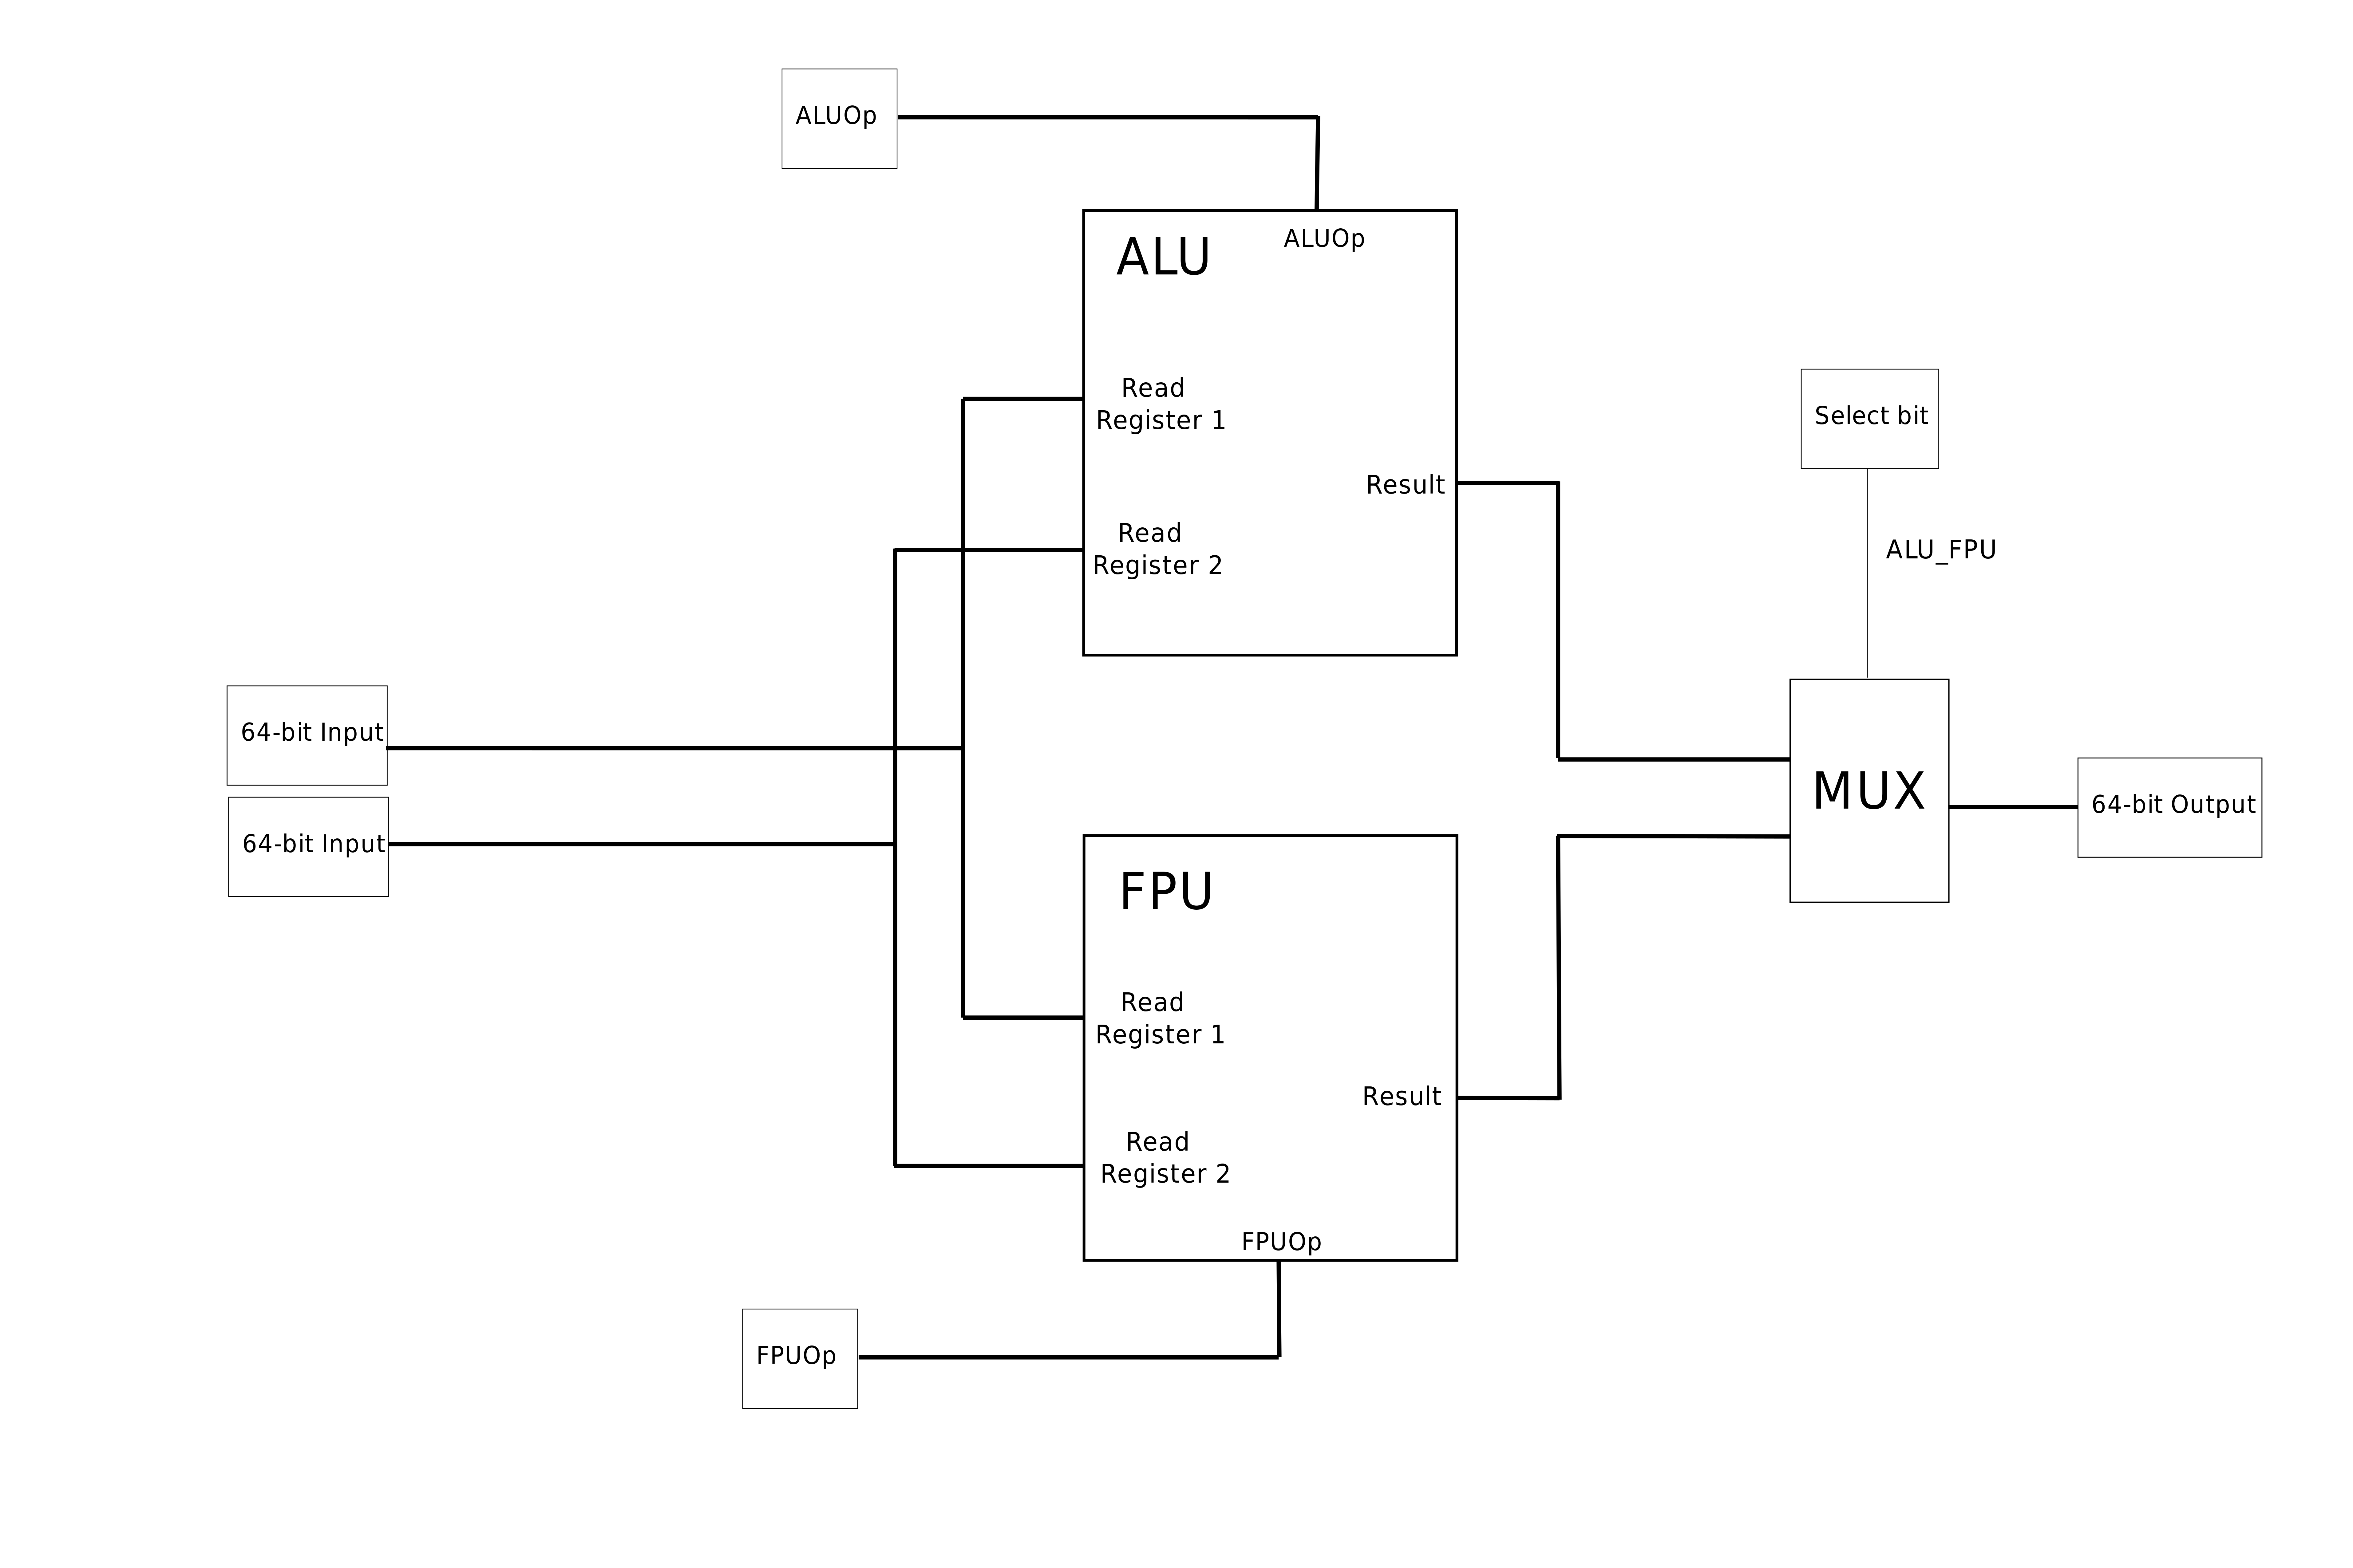
\includegraphics[width=0.7\linewidth]{ALU_FPUblock.png}
    \caption{ALU-FPU block as a whole}
    \label{fig:placeholder}
\end{figure}


\section*{Explaining the Datapath}

\begin{figure}[H]
    \centering
    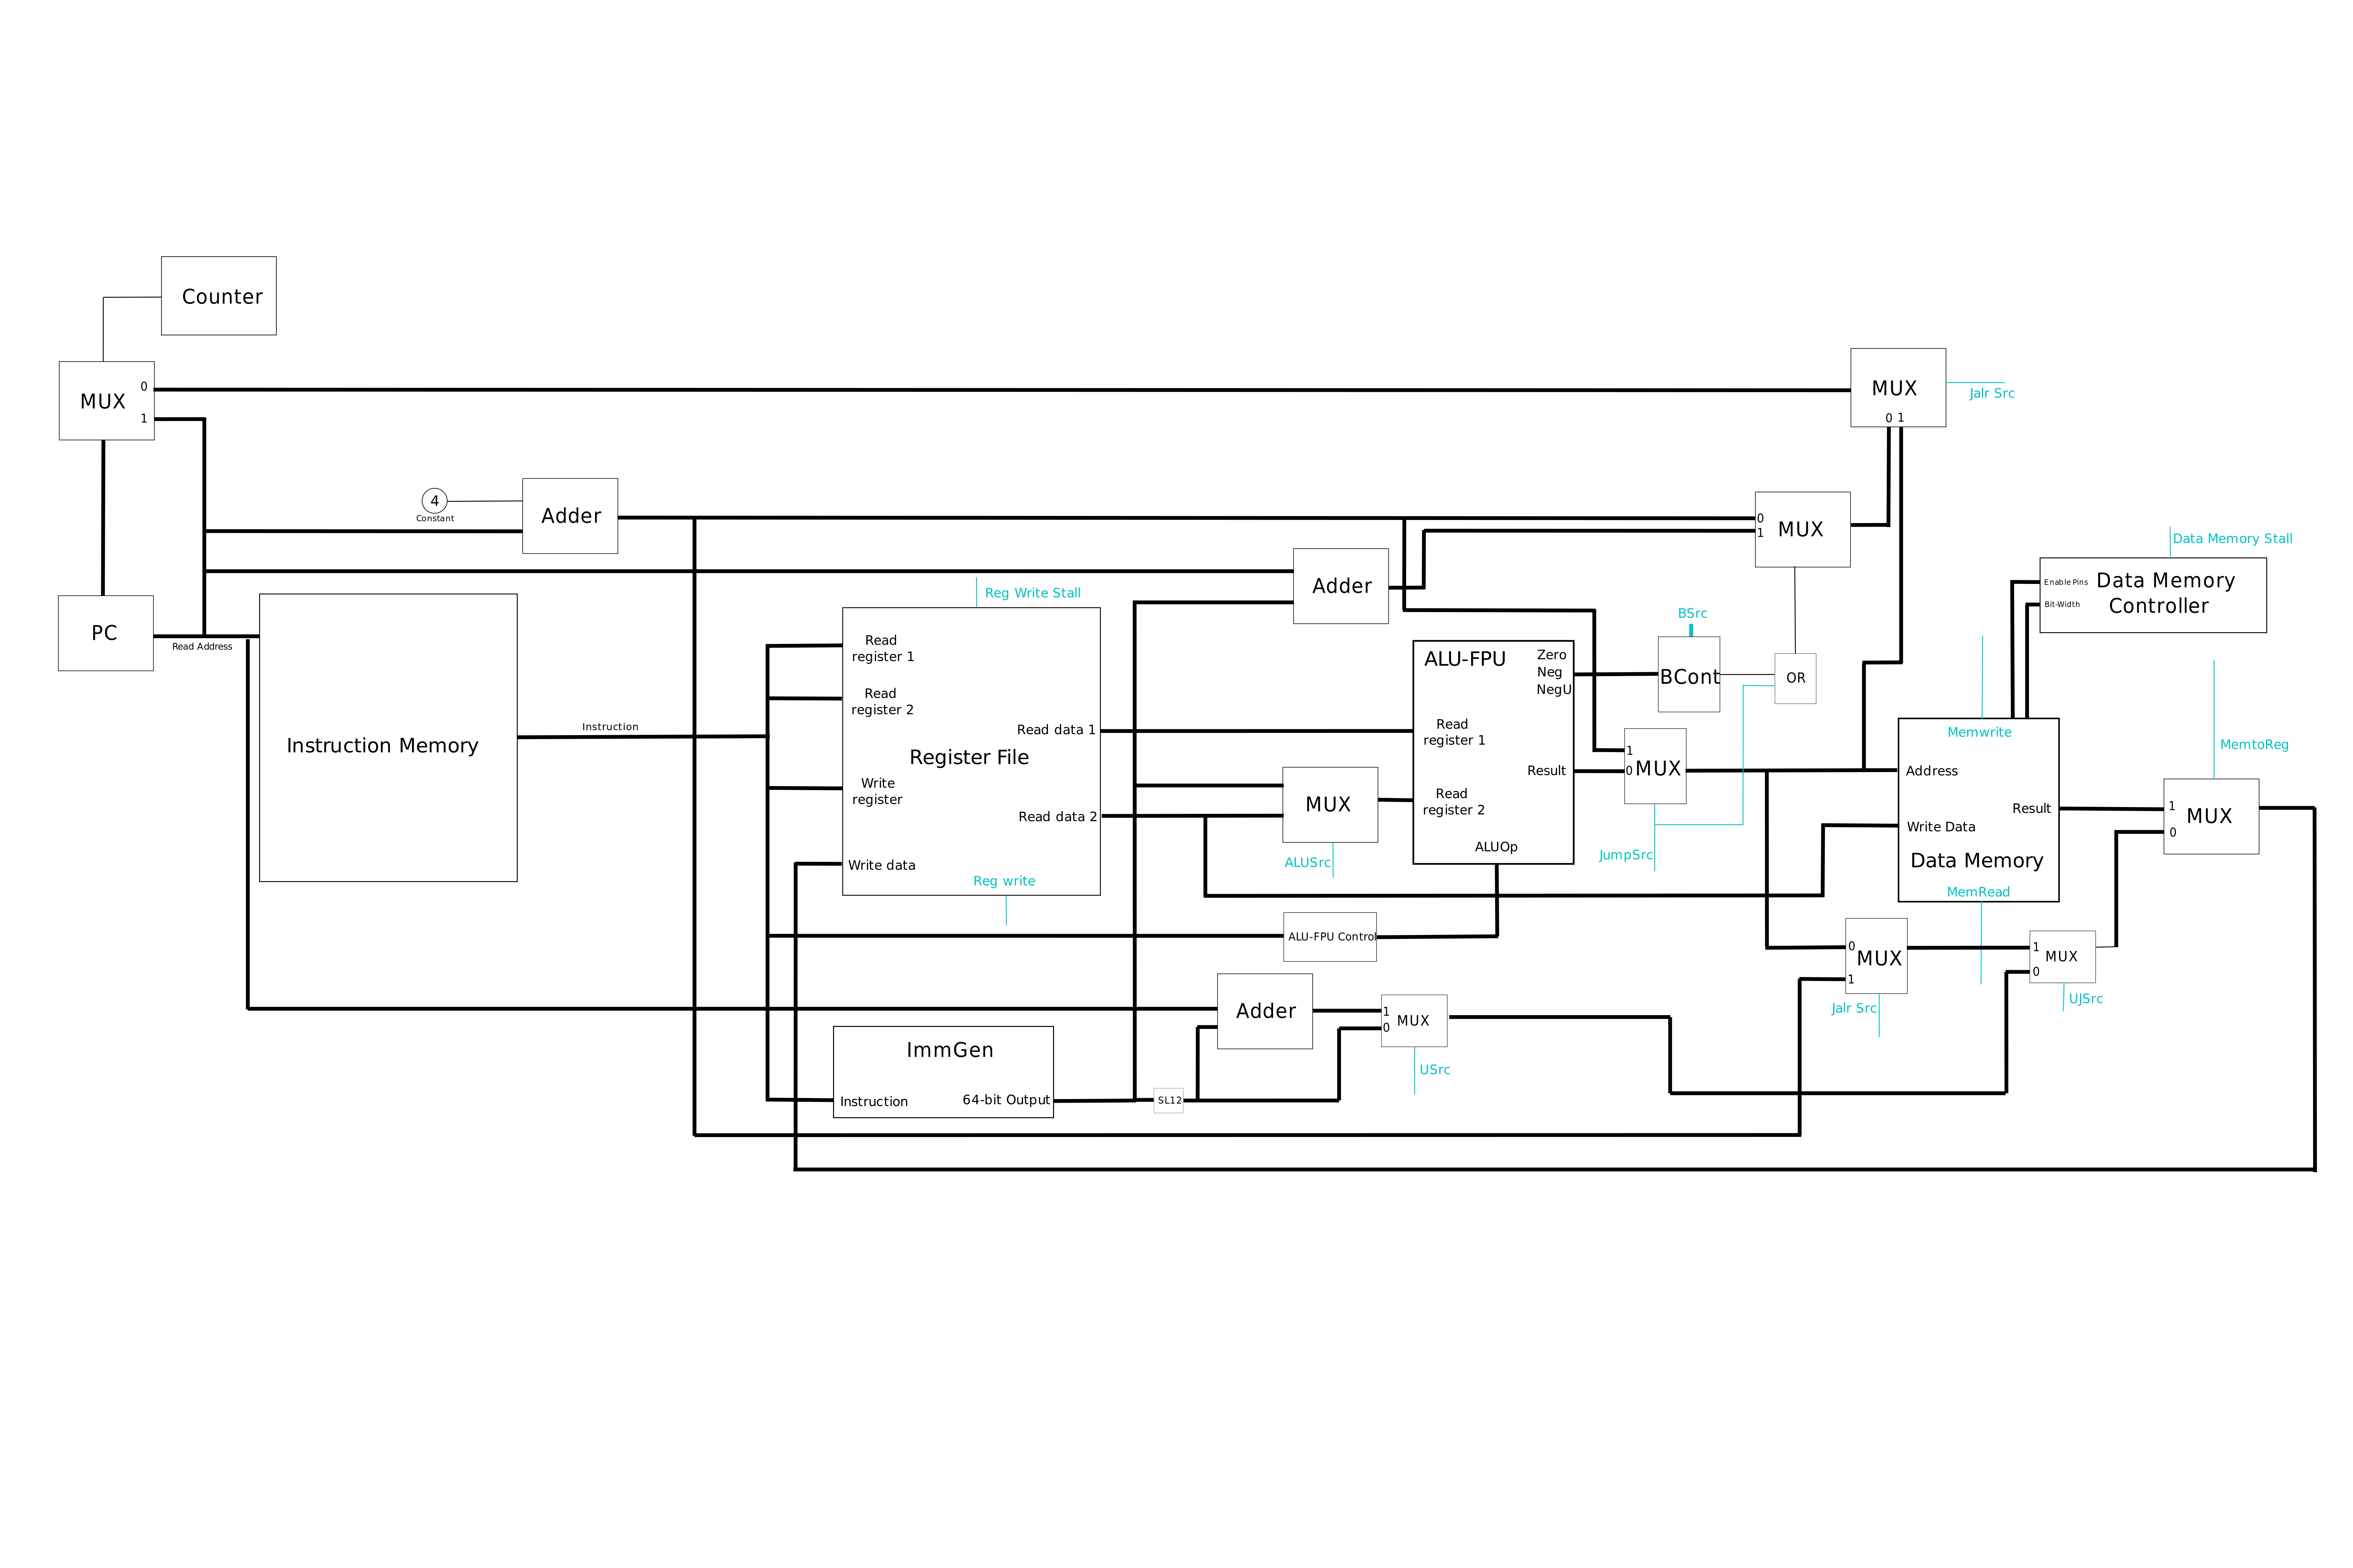
\includegraphics[width=\linewidth]{datapath.png}
    \caption{Complete Single-Cycle Processor Datapath}
    \label{fig:datapath}
\end{figure}

\subsection*{R-format Instruction Path}

\begin{itemize}
    \item R-format instructions execute through a well-defined datapath sequence. The instruction is first retrieved from the Instruction Memory, where the bits corresponding to the source and destination registers are extracted and forwarded to the Register File. The Register File outputs the values stored in the specified source registers.

    \item The Control Unit (not shown in the diagram) configures the \texttt{ALUSrc} control signal such that the multiplexer selects the source register value rather than an immediate. These operands are then routed to the ALU-FPU block, where the ALU-FPU control signals determine the specific arithmetic or logical operation to be performed. The ALU-FPU output is connected to the address port of the Data Memory; however, the \texttt{MemRead} and \texttt{MemWrite} control signals remain deasserted to prevent unintended memory modifications.

    \item The ALU-FPU result is also directed to a multiplexer that selects between the ALU-FPU output and data retrieved from memory. For R-format instructions, the multiplexer select signal is configured to choose the ALU-FPU output, which is then written to the destination register by asserting the \texttt{RegWrite} control signal in the Register File.
\end{itemize}

\subsection*{I-format Instruction Path}

\begin{itemize}
    \item Similar to R-format instructions, the I-format instruction is first retrieved from the Instruction Memory, where the bits corresponding to the source and destination registers are extracted and forwarded to the Register File. The Register File outputs the values stored in the specified source registers.

    \item The Control Unit configures the \texttt{ALUSrc} control signal such that the multiplexer selects the immediate value rather than the source register value. These operands are then routed to the ALU-FPU block, where the ALU-FPU control signals determine the specific arithmetic or logical operation to be performed. The ALU-FPU output is connected to the address port of the Data Memory. For load operations, the \texttt{MemRead} control signal is asserted while the \texttt{MemWrite} control signal remains deasserted to prevent unintended memory modifications.

    \item The ALU-FPU result is directed to a multiplexer that selects between the ALU-FPU output and data retrieved from memory. For load instructions, the multiplexer select signal is configured to choose the memory output, which is then written to the destination register by asserting the \texttt{RegWrite} control signal in the Register File. For non-load I-format instructions, the datapath flow follows the same sequence as R-format instructions.

    \item For the \texttt{jalr} instruction, the value \texttt{PC+4} is forwarded to two multiplexers (controlled by \texttt{JumpSrc} and \texttt{UJSrc} select lines), which configure the destination register to receive \texttt{PC+4}. To compute \texttt{PC = rs1 + imm}, the ALU is utilized. A multiplexer selects between this computed value and \texttt{PC+4} for the next program counter value, with the selection controlled by the \texttt{JalrSrc} signal.
\end{itemize}

\subsection*{B-format Instruction Path}

For B-format instructions, the condition flags from the ALU are utilized instead of the ALU result itself. These flags determine whether \texttt{PC+imm} or \texttt{PC+4} becomes the next program counter value. The branch conditions are evaluated in the Branch Control block (\texttt{BCont}), with the specific branch condition type specified by the \texttt{BSrc} signal from the Control Unit. When the branch condition evaluates to true, the branch control signal is asserted and \texttt{PC+imm} is selected; otherwise, \texttt{PC+4} is selected to continue sequential execution.

\subsection*{J-format Instruction Path}

The execution process for J-format instructions is nearly identical to the \texttt{jalr} instruction, except that instead of using the ALU to compute \texttt{rs1 + imm}, a dedicated adder with inputs \texttt{PC} and \texttt{imm} is employed to calculate the target address.

\subsection*{S-format Instruction Path}

For S-format instructions, the effective address \texttt{rs1 + imm} is calculated through the ALU block, similar to I-format instructions. The value from register \texttt{rs2} is connected to the Write Data port of the Data Memory, and the \texttt{MemWrite} control signal is asserted to write the data to memory at the computed address.

\subsection*{U-format Instruction Path}

A dedicated adder is placed adjacent to the immediate generation block. After the generated immediate is shifted left by 12 bits, a multiplexer controlled by the \texttt{USrc} signal selects between the two U-format operations: \texttt{lui} (load upper immediate) loads the shifted immediate directly, while \texttt{auipc} (add upper immediate to PC) adds the shifted immediate to the current program counter value.

\section*{Register File}

The Register File contains 64 registers: the first 32 serve as general-purpose integer registers, while the next 32 are dedicated to floating-point operations. Register addresses are extracted from the instruction encoding. For floating-point instructions, the appropriate register is selected by adding 32 to the specified address. For integer instructions, the address is used directly without modification. To support this addressing scheme, a small adder computes the offset by adding 32 to the register address field. A multiplexer then selects between the original address and the offset address based on a control signal from the Control Unit, which indicates whether the instruction operates on integer or floating-point registers.

\section*{Data Memory}

\begin{figure}[H]
    \centering
    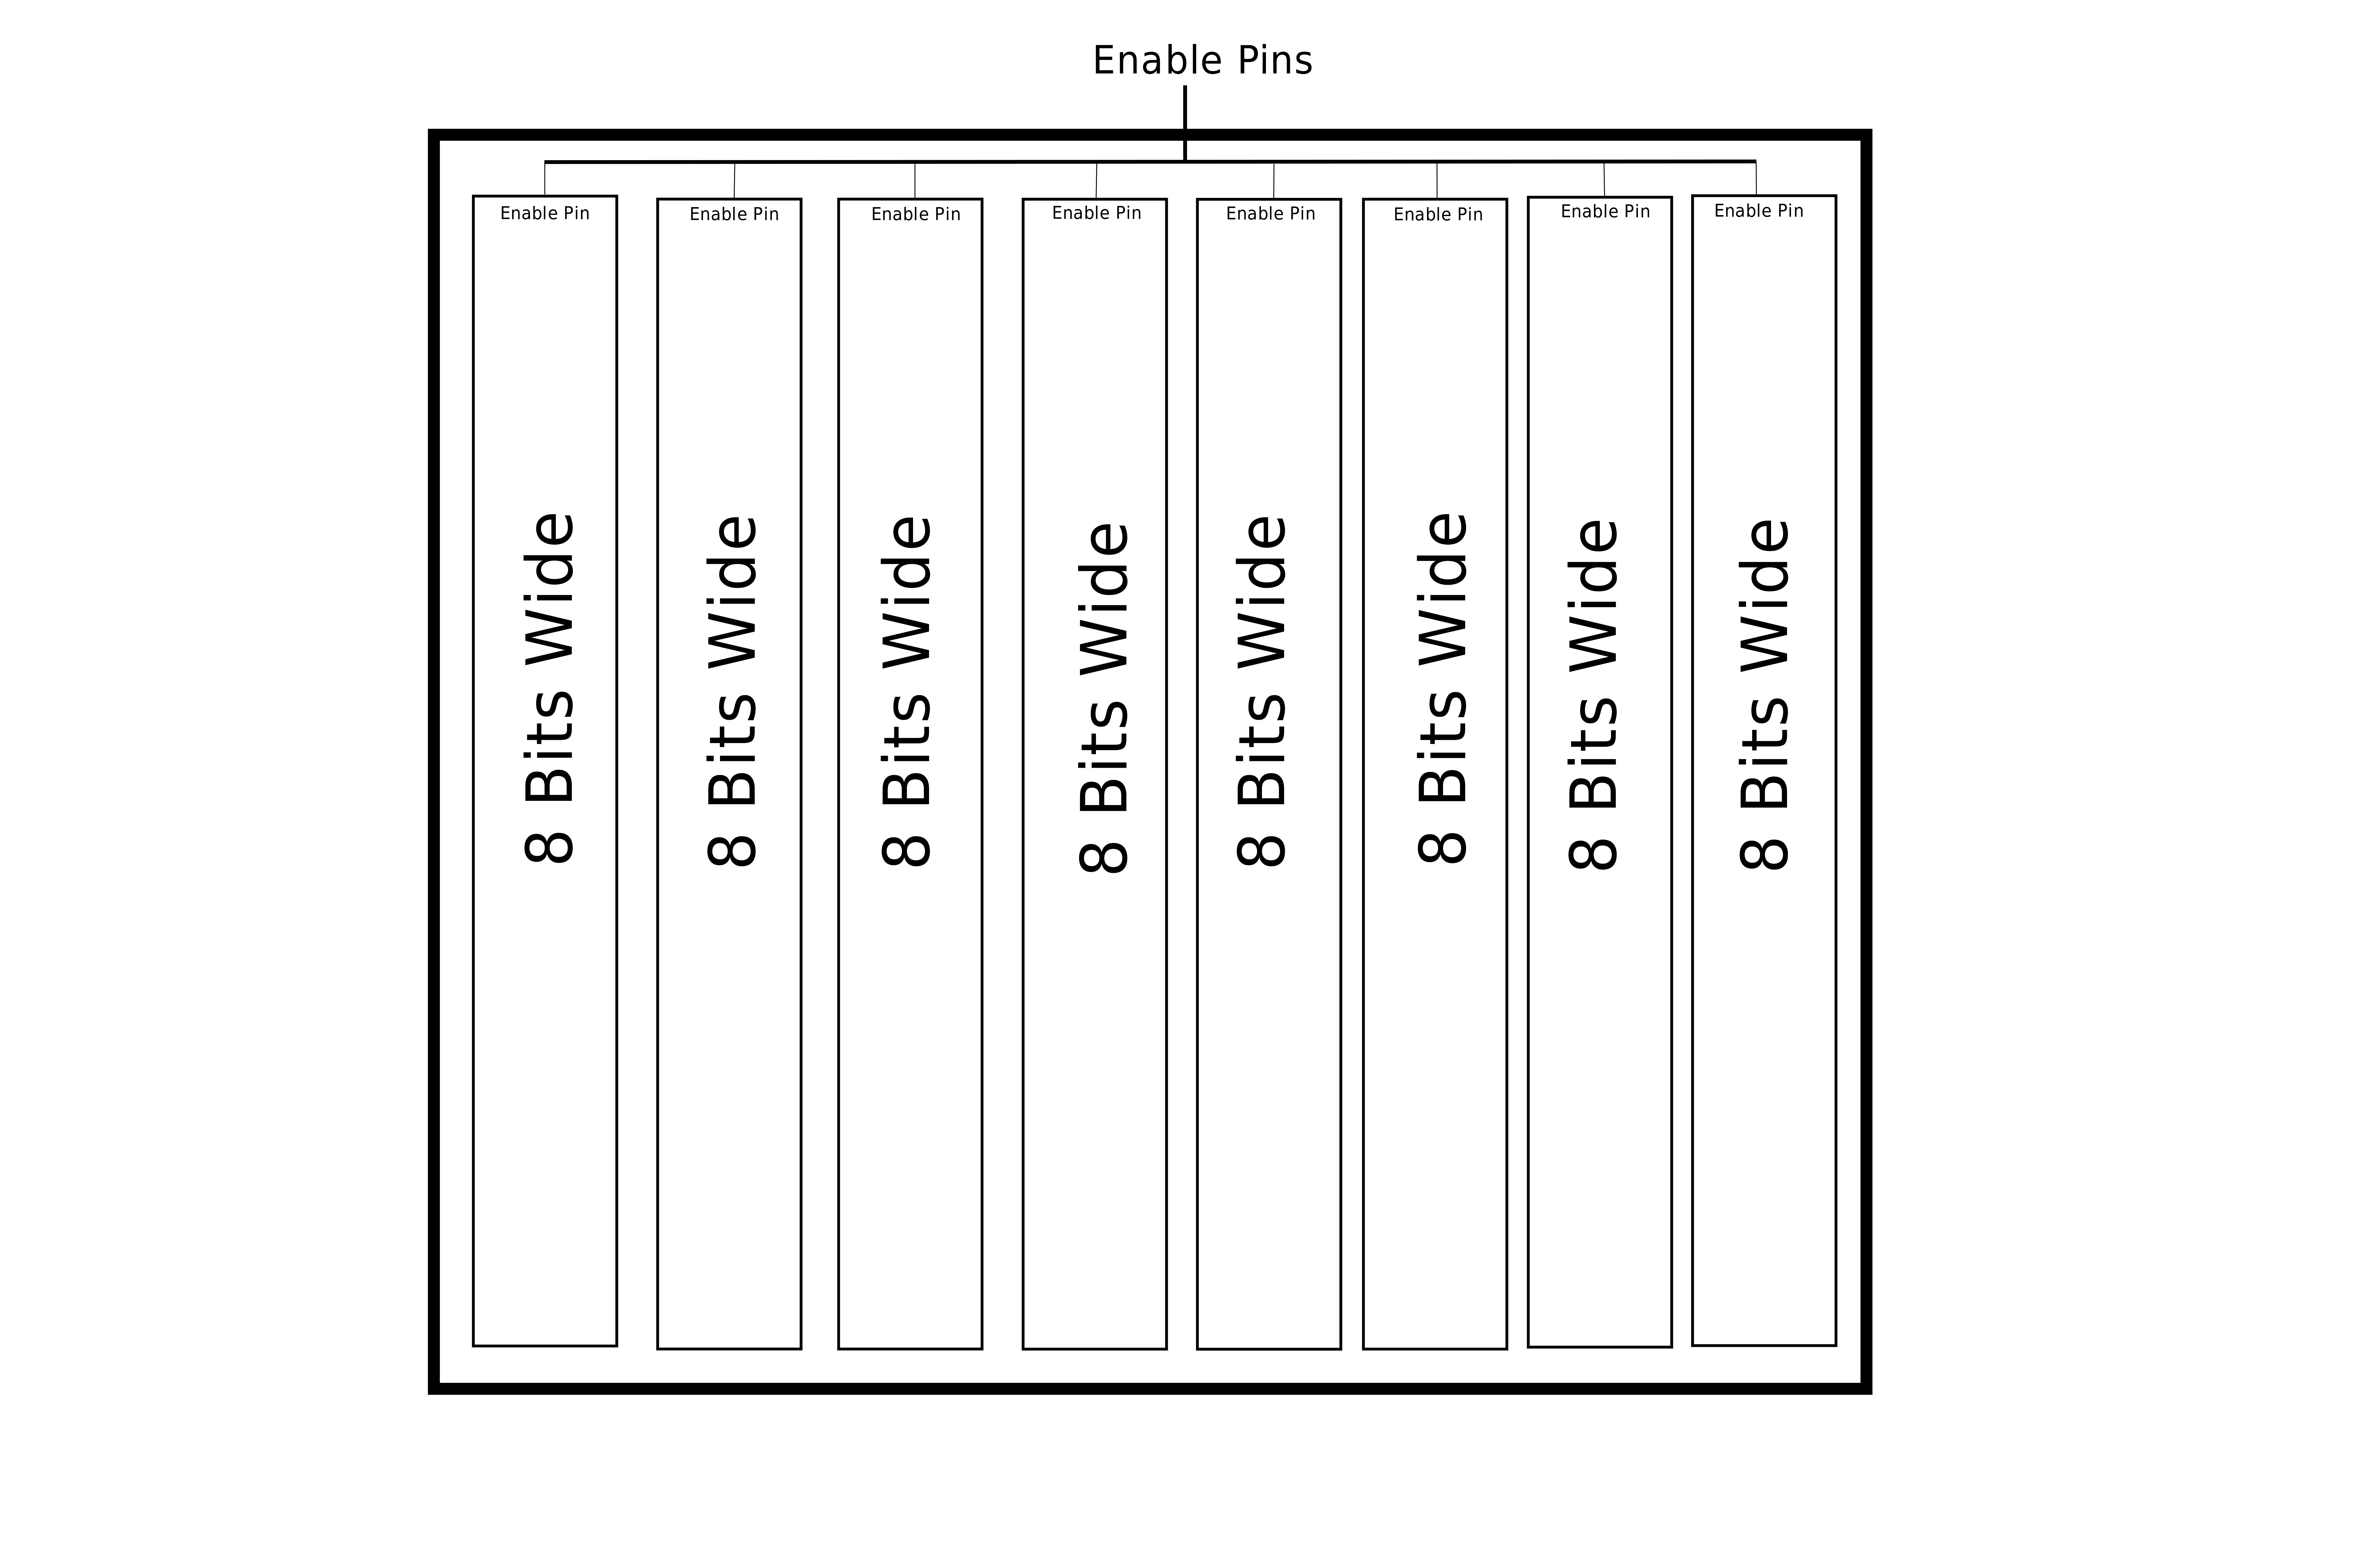
\includegraphics[width=0.7\textwidth]{data_memory.png}
    \caption{Data Memory Architecture}
    \label{fig:data_memory}
\end{figure}

\subsection*{Memory Organization}

The Data Memory block is organised into eight parallel sub-blocks, each 8 bits wide. This parallel architecture leverages the physical characteristics of Block RAM (BRAM) on the PYNQ FPGA board to achieve optimal performance.

\subsection*{Address Mapping and Data Placement}

The lower three bits of the memory address determine which sub-block receives the data. Specifically, when the address bits \texttt{[2:0]} equal \texttt{000}, data is stored in the first block; when \texttt{001}, data is stored in the second block, and so forth through all eight blocks. The number of sub-blocks utilized depends on the data width specified by the instruction:

\begin{itemize}
    \item \textbf{Byte operations} (\texttt{lb}, \texttt{sb}): Utilize 1 sub-block (8 bits)
    \item \textbf{Half-word operations} (\texttt{lh}, \texttt{sh}): Utilize 2 sub-blocks (16 bits)
    \item \textbf{Word operations} (\texttt{lw}, \texttt{sw}): Utilize 4 sub-blocks (32 bits)
    \item \textbf{Double-word operations} (\texttt{ld}, \texttt{sd}): Utilize 8 sub-blocks (64 bits)
\end{itemize}

When a memory access requires storing data beyond the eighth sub-block (address bits \texttt{[2:0]} exceeding \texttt{111}), the addressing wraps around to the first sub-block, maintaining the circular nature of the 8-block architecture.

\subsection*{Performance Advantages}

This parallel memory architecture is specifically designed to exploit the pipelined nature of BRAM on the PYNQ board. In a conventional linear memory arrangement, the pipelined BRAM requires two clock cycles to retrieve a single byte, resulting in memory operations taking more than three cycles to complete.

The implemented 8-way parallel architecture significantly reduces this latency. Memory load and store operations are now complete in a maximum of three clock cycles in the worst case, with many operations completing faster depending on alignment. This design choice provides substantial performance improvements for memory-intensive operations while maintaining compatibility with the RISC-V memory model. To support this two cycle stall, a small counter is used near the PC update point such that when the counter is not in the initial configuration, the PC will remain the same, turn off the changes in the register file through an enable. This has not been implemented yet.

\subsection*{Initial Idea}
The initial design approach utilised a similar parallel sub-block architecture as described below, but with a significant constraint: all data, regardless of its size, was required to be stored starting from a memory location where the lower three address bits were \texttt{000}. While this alignment simplification eased the initial implementation, it introduced substantial inefficiencies. This approach wasted considerable memory space by leaving gaps between non-aligned accesses. Furthermore, it failed to accurately model real-world memory behavior, where data can overlap and occupy any byte-aligned address. The inability to support arbitrary byte addressing was a fundamental limitation that necessitated a redesign to properly implement the RISC-V memory model.

\section*{Conclusion}

The fundamental arithmetic and logic components of the RV64IM processor have been successfully designed and implemented. These units form the execution core that will be integrated into the complete datapath. The modular design approach allows for thorough testing at each level and will facilitate the transition to a pipelined architecture in Phase 2 of the project.

\end{document}


